\documentclass{article}

\usepackage{amsmath}
\usepackage{graphicx}
\usepackage[colorlinks,allcolors=blue]{hyperref}
\usepackage{cleveref}

\begin{document}

\title{Composite Section Properties}
\author{Andrew Ning}
\date{}
\maketitle

\section{Constitutive Equations}

Assuming a linearly elastic material, the most general relationship between the stress tensor and the strain tensor is:
\begin{equation}
\sigma_{ij} = K_{ijkl} \epsilon_{kl},
\label{eq:generalstressstrain}
\end{equation}
where $K_{ijkl}$ is a fourth-order stiffness tensor, which is a function of material properties.  In general this stiffness tensor has $3^4 = 81$ constants.

However, we know that the stress tensor is symmetric:
\begin{equation}
\sigma_{ij} = \sigma_{ji}.
\end{equation}
Using \cref{eq:generalstressstrain} we see that
\begin{align}
\sigma_{ij} &= K_{ijkl} \epsilon_{kl}\\
\sigma_{ji} &= K_{jikl} \epsilon_{kl}.
\end{align}
Equating the two stresses shows that:
\begin{equation}
K_{ijkl} = K_{jikl}.
\end{equation}
Thus, we now have $6 \cdot 3 \cdot 3 = 54$ constants as the $ij$ terms correspond to the 6 unique stress components of a symmetric second-order stress tensor.  Strain exhibits the same symmetry:
\begin{equation}
\epsilon_{kl} = \epsilon_{lk},
\end{equation}
so we have now reduced the number of unique constants to $6 \cdot 6 = 36$.
These two symmetries are referred to as \emph{minor symmetries} ($K_{ijkl} = K_{jikl}$ and $K_{ijkl} = K_{ijlk}$).

We can express symmetric tensors more compactly in matrix or vector notation.  The symmetric stress tensor:
\begin{equation}
\begin{bmatrix}
    \sigma_{11} & \sigma_{12} & \sigma_{13} \\
    \sigma_{21} & \sigma_{22} & \sigma_{23} \\
    \sigma_{31} & \sigma_{32} & \sigma_{33},
\end{bmatrix}
\end{equation}
has only six unique components and so can be expressed as a vector:
\begin{equation}
\begin{bmatrix}
    \sigma_{11} & \sigma_{22} & \sigma_{33} & \sigma_{12} & \sigma_{13} & \sigma_{23}.
\end{bmatrix}
\end{equation}
Similarly, the symmetric strain tensor:
\begin{equation}
\begin{bmatrix}
\epsilon_{11} & \epsilon_{12} & \epsilon_{13} \\
\epsilon_{21} & \epsilon_{22} & \epsilon_{23} \\
\epsilon_{31} & \epsilon_{32} & \epsilon_{33} \\
\end{bmatrix}
\end{equation}
can also be reduced to a vector.  However, the appropriate form is:
\begin{equation}
\begin{bmatrix}
    \epsilon_{11} & \epsilon_{22} & \epsilon_{33} & 2 \epsilon_{12} & 2 \epsilon_{13} & 2 \epsilon_{23}
\end{bmatrix}
\end{equation}
The reason that the factors of 2 appear is that the strain energy density for a linearly elastic material is:
\begin{equation}
\begin{aligned}
\psi &= \frac{1}{2} C_{ijkl} \epsilon_{ij} \epsilon_{kl}\\
&= \frac{1}{2} \sigma_{ij} \epsilon_{ij}
\end{aligned}
\label{eq:strainenergy}
\end{equation}
Using the tensors this equals:
\begin{equation}
\frac{1}{2} \sigma_{11} \epsilon_{11} + \frac{1}{2} \sigma_{22} \epsilon_{22} + \frac{1}{2} \sigma_{33} \epsilon_{33} + \sigma_{12} \epsilon_{12} + \sigma_{13} \epsilon_{13} + \sigma_{23} \epsilon_{23}
\end{equation}
The last three terms were simplified from (showing one of the terms):
\begin{equation}
    \frac{1}{2}\sigma_{12} \epsilon_{12} + \frac{1}{2}\sigma_{21} \epsilon_{21} = \sigma_{12} \epsilon_{12},
\end{equation}
from symmetry in the stress and strain tensors.  Thus, to preserve the correct expression for the strain energy when using the vector forms:
\begin{equation}
\psi = \frac{1}{2} \sigma_i \epsilon_i,
\end{equation}
we need to include the factor of 2 in one of the terms.  We include it in the strain term because the strain energy is typically expressed just in terms of the strain as shown in the first expression on \cref{eq:strainenergy}.

We have now reduced both the stress and strain tensors to vectors.  We can also reduce the fourth order stiffness tensor.  Any fourth order tensor with minor symmetry can be expressed as a 6 $\times$ 6 matrix.  In our case this is done as follows:
\begin{equation}
\left[
\begin{matrix}
\sigma_{11}\\
\sigma_{22}\\
\sigma_{33}\\
\tau_{12}\\
\tau_{13}\\
\tau_{23}
\end{matrix}
\right]
=
\left[
\begin{matrix}
K_{1111} & K_{1122} & K_{1133} & K_{1112} & K_{1113} & K_{1123} \\
K_{2211} & K_{2222} & K_{2233} & K_{2212} & K_{2213} & K_{2223} \\
K_{3311} & K_{3322} & K_{3333} & K_{3312} & K_{3313} & K_{3323} \\
K_{1211} & K_{1222} & K_{1233} & K_{1212} & K_{1213} & K_{1223} \\
K_{1311} & K_{1322} & K_{1333} & K_{1312} & K_{1313} & K_{1323} \\
K_{2311} & K_{2322} & K_{2333} & K_{2312} & K_{2313} & K_{2323} \\
\end{matrix}
\right]
\left[
\begin{matrix}
\epsilon_{11}\\
\epsilon_{22}\\
\epsilon_{33}\\
2 \epsilon_{12}\\
2 \epsilon_{13}\\
2 \epsilon_{23}
\end{matrix}
\right].
\label{eq:constitutive1}
\end{equation}

We can reduce the number of necessary constants further.  The stress can also be defined as the derivative of the strain energy with respect to strain:
\begin{equation}
\sigma_{ij} = \frac{\partial \psi}{\partial \epsilon_{ij}}
\end{equation}
If we now take second derivatives of the strain energy we get:
\begin{equation}
\frac{\partial^2 \psi}{\partial \epsilon_{kl} \partial \epsilon_{ij}} = \frac{\partial}{\partial_{kl}} \left( \sigma_{ij} \right) = \frac{\partial}{\partial_{kl}} \left( C_{ijmn} \epsilon_{mn}\right) = C_{ijkl}
\end{equation}
However, the mixed partials of second derivatives must be equal so:
\begin{equation}
\frac{\partial^2 \psi}{\partial \epsilon_{ij} \partial \epsilon_{kl}} = \frac{\partial}{\partial \epsilon_{ij}} \left( \sigma_{kl} \right) = \frac{\partial}{\partial_{ij}} \left( C_{klmn} \epsilon_{mn}\right) = C_{klij}
\end{equation}
Thus, $C_{ijkl} = C_{klij}$, which is called \emph{major symmetry}.  We have thus reduced to 21 material constants (i.e., the matrix in \cref{eq:constitutive1} is symmetric, so for example, $K_{1133} = K_{3311}$).

Since we are using a matrix form it is more convenient to use just two indices, rather than preserve the tensor notation.  Thus, we map $_{11}$ to $_{1}$, $_{12}$ to $_{4}$ and so on.  Furthermore, we will use the engineering shear strains: $\gamma_{12} = 2 \epsilon_{12}$ for convenience to remove the factors of 2.
\begin{equation}
\left[
\begin{matrix}
\sigma_{11}\\
\sigma_{22}\\
\sigma_{33}\\
\tau_{12}\\
\tau_{13}\\
\tau_{23}
\end{matrix}
\right]
=
\left[
\begin{matrix}
K_{11} & K_{12} & K_{13} & K_{14} & K_{15} & K_{16} \\
K_{21} & K_{22} & K_{23} & K_{24} & K_{25} & K_{26} \\
K_{31} & K_{32} & K_{33} & K_{34} & K_{35} & K_{36} \\
K_{41} & K_{42} & K_{43} & K_{44} & K_{45} & K_{46} \\
K_{51} & K_{52} & K_{53} & K_{54} & K_{55} & K_{56} \\
K_{61} & K_{62} & K_{63} & K_{64} & K_{65} & K_{66}
\end{matrix}
\right]
\left[
\begin{matrix}
\epsilon_{11}\\
\epsilon_{22}\\
\epsilon_{33}\\
\gamma_{12}\\
\gamma_{13}\\
\gamma_{23}
\end{matrix}
\right]
\end{equation}
Often for convenience the double repeated subscripts are dropped for the stresses and strain ($\sigma_1$ instead of $\sigma_{11}$) and we will adopt this as well.

% or
% \begin{equation}
% \boldsymbol{\sigma} = \boldsymbol{K} \boldsymbol{\epsilon}
% \end{equation}
% where $K$ is called the stiffness matrix and can be shown to be symmetric.

Thus, in this general case there are 21 independent constants needed to define the material properties.
These are called the \emph{constitutive relationships} and can also be written as the inverse mapping:
\begin{equation}
\boldsymbol{\epsilon} = \boldsymbol{S} \boldsymbol{\sigma}
\end{equation}
where $S = K^{-1}$ is the compliance matrix.  The compliance matrix is also symmetric since the inverse of a symmetric matrix is also symmetric.

Usually, a material has certain symmetries.  \emph{Orthotropic} materials have three orthogonal planes of symmetry and in that case the stiffness matrix can be reduced to:
\begin{equation}
\left[
\begin{matrix}
\sigma_{1}\\
\sigma_{2}\\
\sigma_{3}\\
\tau_{12}\\
\tau_{13}\\
\tau_{23}
\end{matrix}
\right]
=
\left[
\begin{matrix}
K_{11} & K_{12} & K_{13} & 0 & 0 & 0 \\
K_{21} & K_{22} & K_{23} & 0 & 0 & 0 \\
K_{31} & K_{32} & K_{33} & 0 & 0 & 0 \\
0 & 0 & 0 & K_{44} & 0 & 0 \\
0 & 0 & 0 & 0 & K_{55} & 0 \\
0 & 0 & 0 & 0 & 0 & K_{66}
\end{matrix}
\right]
\left[
\begin{matrix}
\epsilon_{1}\\
\epsilon_{2}\\
\epsilon_{3}\\
\gamma_{12}\\
\gamma_{13}\\
\gamma_{23}
\end{matrix}
\right]
\label{eq:orthoconstit}
\end{equation}
There are now only 9 unknown constants.  These constants are functions of the following 9 material properties: $E_{1}$, $E_{2}$, $E_{3}$, $G_{12}$, $G_{13}$, $G_{23}$, $\nu_{12}$, $\nu_{13}$, $\nu_{23}$, where ${E}_{i}$ is the Young's modulus along axis i, $G_{ij}$ is the shear modulus in direction j on the plane whose normal is in direction i, and $\nu_{ij}$ is the Poisson's ratio that corresponds to a contraction in direction j when an extension is applied in direction i.

These relationships are more compactly represented in the compliance matrix as opposed to the stiffness matrix:
\begin{equation}
\left[
\begin{matrix}
\epsilon_{1}\\
\epsilon_{2}\\
\epsilon_{3}\\
\gamma_{12}\\
\gamma_{13}\\
\gamma_{23}
\end{matrix}
\right]
=
\left[
\begin{matrix}
\frac{1}{E_1} & \frac{-\nu_{21}}{E_2} & \frac{-\nu_{31}}{E_3} & 0 & 0 & 0 \\
\frac{-\nu_{12}}{E_1} & \frac{1}{E_2} & \frac{-\nu_{32}}{E_3} & 0 & 0 & 0 \\
\frac{-\nu_{13}}{E_1} & \frac{-\nu_{23}}{E_2} & \frac{1}{E_3} & 0 & 0 & 0 \\
0 & 0 & 0 & \frac{1}{G_{12}} & 0 & 0 \\
0 & 0 & 0 & 0 & \frac{1}{G_{13}} & 0 \\
0 & 0 & 0 & 0 & 0 & \frac{1}{G_{23}}
\end{matrix}
\right]
\left[
\begin{matrix}
\sigma_{1}\\
\sigma_{2}\\
\sigma_{3}\\
\tau_{12}\\
\tau_{13}\\
\tau_{23}
\end{matrix}
\right]
\label{eq:orthocompliance}
\end{equation}

From symmetry we see that, for example,:
\begin{equation}
\frac{\nu_{21}}{E_2} = \frac{\nu_{12}}{E_1}
\end{equation}
Or, expressing all three relationships compactly in index notation we have:
\begin{equation}
\nu_{ij} E_j = \nu_{ji} E_i
\label{eq:nue}
\end{equation}

The inverse of the matrix is a bit more cumbersome, but is given as:
\begin{equation}
\left[
\begin{matrix}
\sigma_{1}\\
\sigma_{2}\\
\sigma_{3}\\
\tau_{12}\\
\tau_{13}\\
\tau_{23}
\end{matrix}
\right]
=
\left[
\begin{matrix}
E_1(1 - \nu_{23}\nu_{32})\Delta & E_1(\nu_{21} + \nu_{31}\nu_{23})\Delta & E_1(\nu_{31} + \nu_{21}\nu_{32})\Delta & 0 & 0 & 0 \\
E_2(\nu_{12} + \nu_{32}\nu_{13})\Delta & E_2(1 - \nu_{13}\nu_{31})\Delta & E_2(\nu_{32} + \nu_{12}\nu_{31})\Delta & 0 & 0 & 0 \\
E_3(\nu_{13} + \nu_{12}\nu_{23})\Delta & E_3(\nu_{23} + \nu_{13}\nu_{21})\Delta & E_3(1 - \nu_{12}\nu_{21})\Delta & 0 & 0 & 0 \\
0 & 0 & 0 & G_{12} & 0 & 0 \\
0 & 0 & 0 & 0 & G_{13} & 0 \\
0 & 0 & 0 & 0 & 0 & G_{23}
\end{matrix}
\right]
\left[
\begin{matrix}
\epsilon_{1}\\
\epsilon_{2}\\
\epsilon_{3}\\
\gamma_{12}\\
\gamma_{13}\\
\gamma_{23}
\end{matrix}
\right]
\label{eq:orthostiffness}
\end{equation}
where
\begin{equation}
\Delta = \frac{1}{1 - \nu_{12}\nu_{21} - \nu_{23}\nu_{32} - \nu_{31}\nu_{13} - 2\nu_{21}\nu_{32}\nu_{13}}
\end{equation}

Composites are generally made of layers of orthotropic materials so this form will be the starting point for the stiffness of an individual ply.

\section{Change of Basis}

Consider the stress tensor (or any second order tensor) written as:
\begin{equation}
\sigma = \sigma_{ij} e_i \otimes e_j
\label{eq:unrotated}
\end{equation}
where $\otimes$ is an outer product and $e_i$ is a unit vector in the $i^{\text{th}}$ direction.
We would like to express this tensor in a different coordinate system $e_i^\prime$:
\begin{equation}
    \sigma = \sigma^\prime_{ij} e^\prime_i \otimes e^\prime_j
\end{equation}
and now need to determine how the components $\sigma^\prime$ relate to the original components of the stress tensor.

These are two representations of the same tensor, so they must be equivalent:
\begin{equation}
    \sigma_{ij} e_i \otimes e_j = \sigma^\prime_{ij} e^\prime_i \otimes e^\prime_j
\end{equation}
We multiply both with left and right vector products using the new basis vectors.   This would be a vector-matrix-vector product against the original tensor in matrix form, or in the basis representation it is two dot products:
\begin{align}
    {e^\prime_i}^T \left[ \sigma_{kl} e_k \otimes e_l \right] e^\prime_j &= {e^\prime_i}^T \left[ \sigma^\prime_{ij} e^\prime_i \otimes e^\prime_j \right] e^\prime_j\\
    \sigma_{kl} (e^\prime_i \cdot e_k) (e^\prime_j \cdot e_l) &= \sigma^\prime_{ij} (e^\prime_i \cdot e^\prime_i) (e^\prime_j \cdot e^\prime_j)\\
    \sigma_{kl} (e^\prime_i \cdot e_k) (e^\prime_j \cdot e_l) &= \sigma^\prime_{ij}
\end{align}
This provides the needed transformation with the dot products as directions cosines of the angles between $e_i$ and $e^\prime_j$, for example.

If we express the direction cosines in matrix form: $R_{ij} = e_i^\prime \cdot e_j$ then we express the rotation as:
\begin{equation}
\sigma^\prime_{ij} = R_{ik} R_{jl} \sigma_{kl}
\label{eq:sigmatensor}
\end{equation}
or in matrix form:
\begin{equation}
\sigma^\prime = R \sigma R^T
\end{equation}
where
\begin{equation}
    R =
    \begin{bmatrix}
        e_1^\prime \cdot e_1 & e_1^\prime \cdot e_2 & e_1^\prime \cdot e_3 \\
        e_2^\prime \cdot e_1 & e_2^\prime \cdot e_2 & e_2^\prime \cdot e_3 \\
        e_3^\prime \cdot e_1 & e_3^\prime \cdot e_2 & e_3^\prime \cdot e_3
    \end{bmatrix}
    \label{eq:Rmatrix}
\end{equation}

The transformation is straightforward in tensor form, or with the stresses expressed as a matrix.  However, we often express the unique components of the stress as vectors, as explained earlier. We would like to provide a matrix transformation in this form.  This is a bit tedious, but can be done directly by mapping the tensor notation to corresponding indices in the vector representation.

We expand the tensor transformation formula, in three dimensions, with a general rotation matrix.  We begin with just the $_{11}$ stress:
\begin{equation}
\begin{aligned}
\sigma_{11}^\prime &= R_{11} \sigma_{11} R_{11} + R_{11} \sigma_{12} R_{12} + R_{11} \sigma_{13} R_{13} + R_{12} \sigma_{21} R_{11} + R_{12} \sigma_{22} R_{12} \\
& + R_{12} \sigma_{23} R_{13} + R_{13} \sigma_{31} R_{11} + R_{13} \sigma_{32} R_{12} + R_{13} \sigma_{33} R_{13}\\
&= R_{11}^2 \sigma_{11} + R_{12}^2 \sigma_{22} + R_{13}^2 \sigma_{33} + 2 R_{11} R_{12} \sigma_{12} + 2 R_{11} R_{13} \sigma_{13} + 2 R_{12} R_{13} \sigma_{23}
\end{aligned}
\end{equation}
We have to repeat this for each stress, but we will do so directly in matrix form following the pattern.  The above equation corresponds to the first row.
\begin{equation}
\begin{bmatrix}
\sigma_1^\prime \\
\sigma_2^\prime \\
\sigma_3^\prime \\
\tau_{12}^\prime \\
\tau_{13}^\prime \\
\tau_{23}^\prime
\end{bmatrix}
=
\begin{bmatrix}
R_{11}^2 & R_{12}^2 & R_{13}^2 & 2 R_{11}R_{12} & 2 R_{11}R_{13} & 2 R_{12}R_{13} \\
R_{21}^2 & R_{22}^2 & R_{23}^2 & 2 R_{21}R_{22} & 2 R_{21}R_{23} & 2 R_{22}R_{23} \\
R_{31}^2 & R_{32}^2 & R_{33}^2 & 2 R_{31}R_{32} & 2 R_{31}R_{33} & 2 R_{32}R_{33} \\
R_{11}R_{21} & R_{12}R_{22} & R_{13}R_{23} & R_{11}R_{22} + R_{12}R_{21} & R_{11}R_{23} + R_{13}R_{21} & R_{12}R_{23} + R_{13}R_{22} \\
R_{11}R_{31} & R_{12}R_{32} & R_{13}R_{33} & R_{11}R_{32} + R_{12}R_{31} & R_{11}R_{33} + R_{13}R_{31} & R_{12}R_{33} + R_{13}R_{32} \\
R_{21}R_{31} & R_{22}R_{32} & R_{23}R_{33} & R_{21}R_{32} + R_{22}R_{31} & R_{21}R_{33} + R_{23}R_{31} & R_{22}R_{33} + R_{23}R_{32} \\
\end{bmatrix}
\begin{bmatrix}
\sigma_1 \\
\sigma_2 \\
\sigma_3 \\
\tau_{12} \\
\tau_{13} \\
\tau_{23}
\end{bmatrix}
\label{eq:Tsigma}
\end{equation}
This provides the desired transformation matrix, which we will call $T_\sigma$.  Thus, with the unique components of the stresses represented in vector form we have:
\begin{equation}
\sigma^\prime = T_\sigma \sigma
\end{equation}
Because we will use the components of this matrix again, we divide it into 3x3 submatrices:
\begin{equation}
T_\sigma =
\begin{bmatrix}
    T_1 & 2 T_2 \\
    T_3 & T_4 \\
\end{bmatrix}
\end{equation}
where
\begin{equation}
T_1 = \begin{bmatrix}
    R_{11}^2 & R_{12}^2 & R_{13}^2 \\
    R_{21}^2 & R_{22}^2 & R_{23}^2 \\
    R_{31}^2 & R_{32}^2 & R_{33}^2
\end{bmatrix}
\end{equation}
\begin{equation}
T_2 = \begin{bmatrix}
    R_{11}R_{12} & R_{11}R_{13} & R_{12}R_{13} \\
    R_{21}R_{22} & R_{21}R_{23} & R_{22}R_{23} \\
    R_{31}R_{32} & R_{31}R_{33} & R_{32}R_{33} \\
\end{bmatrix}
\end{equation}
\begin{equation}
T_3 = \begin{bmatrix}
    R_{11}R_{21} & R_{12}R_{22} & R_{13}R_{23} \\
    R_{11}R_{31} & R_{12}R_{32} & R_{13}R_{33} \\
    R_{21}R_{31} & R_{22}R_{32} & R_{23}R_{33} \\
\end{bmatrix}
\end{equation}
and
\begin{equation}
T_4 = \begin{bmatrix}
    R_{11}R_{22} + R_{12}R_{21} & R_{11}R_{23} + R_{13}R_{21} & R_{12}R_{23} + R_{13}R_{22} \\
    R_{11}R_{32} + R_{12}R_{31} & R_{11}R_{33} + R_{13}R_{31} & R_{12}R_{33} + R_{13}R_{32} \\
    R_{21}R_{32} + R_{22}R_{31} & R_{21}R_{33} + R_{23}R_{31} & R_{22}R_{33} + R_{23}R_{32} \\
\end{bmatrix}
\end{equation}


We repeat the process for strains.  The tensor equation is the same as for stresses:
\begin{equation}
\epsilon^\prime_{ij} = R_{ik} R_{jl} \epsilon_{kl}
\end{equation}
However, when mapping to a 6x6 matrix a few changes are needed because of our use of engineering strains ($\gamma_{ij} = 2 \epsilon_{ij})$.  We first write it in terms of $\epsilon$ since no changes are needed in that case.
\begin{equation}
\begin{bmatrix}
\epsilon_{11}^\prime \\
\epsilon_{22}^\prime \\
\epsilon_{33}^\prime \\
\epsilon_{12}^\prime \\
\epsilon_{13}^\prime \\
\epsilon_{23}^\prime
\end{bmatrix}
=
\begin{bmatrix}
T_1 & 2T_2 \\
T_3 & T_4 \\
\end{bmatrix}
\begin{bmatrix}
\epsilon_{11} \\
\epsilon_{22} \\
\epsilon_{33} \\
\epsilon_{12} \\
\epsilon_{13} \\
\epsilon_{23}
\end{bmatrix}
\end{equation}
We now multiply both sides of the bottom three equations by 2.
\begin{equation}
\begin{bmatrix}
\epsilon_{11}^\prime \\
\epsilon_{22}^\prime \\
\epsilon_{33}^\prime \\
\gamma_{12}^\prime \\
\gamma_{13}^\prime \\
\gamma_{23}^\prime
\end{bmatrix}
=
\begin{bmatrix}
T_1 & 2T_2 \\
2 T_3 & 2 T_4 \\
\end{bmatrix}
\begin{bmatrix}
\epsilon_{11} \\
\epsilon_{22} \\
\epsilon_{33} \\
\epsilon_{12} \\
\epsilon_{13} \\
\epsilon_{23}
\end{bmatrix}
\end{equation}
We now multiply the $\epsilon_{ij}$ terms (shear strains) on the right hand vector by 2 and divide the corresponding columns by 2.
\begin{equation}
\begin{bmatrix}
\epsilon_{11}^\prime \\
\epsilon_{22}^\prime \\
\epsilon_{33}^\prime \\
\gamma_{12}^\prime \\
\gamma_{13}^\prime \\
\gamma_{23}^\prime
\end{bmatrix}
=
\begin{bmatrix}
T_1 & T_2 \\
2T_3 & T_4 \\
\end{bmatrix}
\begin{bmatrix}
\epsilon_{11} \\
\epsilon_{22} \\
\epsilon_{33} \\
\gamma_{12} \\
\gamma_{13} \\
\gamma_{23}
\end{bmatrix}
\end{equation}
When strains are expressed in this vector form we have:
\begin{equation}
\epsilon^\prime = T_\epsilon \epsilon
\end{equation}
where
\begin{equation}
T_\epsilon =
\begin{bmatrix}
    T_1 & T_2 \\
    2 T_3 & T_4 \\
\end{bmatrix}
\label{eq:Tepsilon2}
\end{equation}

For the general case the matrices are not pretty.  The two coordinate systems could be in any orientation relative to each other and so we need a well-defined set of angles, like Euler angles, to describe the rotation.  Fortunately, most of the time rotations occur with a common axis.  In that case, the rotation matrix and the resulting transformation simplifies greatly.  For example, let's consider an example where we rotate about a coincident $z$-axis, with the positive rotation shown in \cref{fig:coordinate}, using the convention for positive ply angles for composites.
\begin{figure}[htbp]
\centering
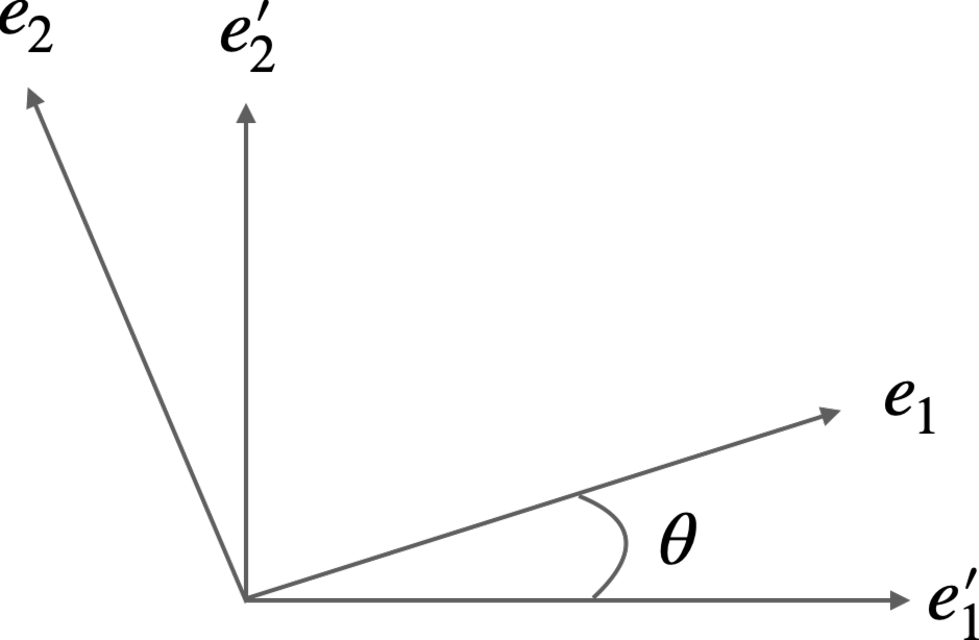
\includegraphics[width=2.0in]{coordinate}
\caption{A rotation between two coordinate axis, with a common $e_3$ axis, which use in our transformation from the unprimed to the primed axes.}
\label{fig:coordinate}
\end{figure}
The axes are related by:
\begin{align}
    \label{eq:transformation}
    e_1^\prime &= e_1 \cos\theta  - e_2 \sin\theta \\
    e_2^\prime &= e_1 \sin\theta  + e_2 \cos\theta \\
    e_3^\prime &= e_3
    \end{align}
The rotation matrix is then (using \cref{eq:Rmatrix}):
\begin{equation}
R =
\begin{bmatrix}
    \cos\theta & -\sin\theta & 0 \\
    \sin\theta & \cos\theta & 0 \\
    0 & 0 & 1 \\
\end{bmatrix}
\end{equation}
The transformation matrix $T_\sigma$ is:
\begin{equation}
    T_\sigma =
\begin{bmatrix}
\cos^2\theta & \sin^2\theta & 0 & -2 \sin\theta\cos\theta & 0 & 0 \\
\sin^2\theta & \cos^2\theta & 0 & 2 \sin\theta\cos\theta &  0  & 0  \\
 0 &  0  &  1  & 0  &  0   &   0   \\
\sin\theta\cos\theta & -\sin\theta\cos\theta & 0  & \cos^2\theta - \sin^2\theta &  0  & 0 \\
 0  & 0  & 0 &  0   & \cos\theta  & -\sin\theta  \\
 0  & 0  &  0   & 0 & \sin\theta  & \cos\theta \\
\end{bmatrix}
\label{eq:rotatezsigma}
\end{equation}
From \cref{eq:Tepsilon2} we can then easily write out $T_\epsilon$ for this case with rotation about the $z$-axis.
\begin{equation}
    T_\epsilon =
\begin{bmatrix}
\cos^2\theta & \sin^2\theta & 0 &  -\sin\theta\cos\theta & 0 & 0 \\
\sin^2\theta & \cos^2\theta & 0 & \sin\theta\cos\theta &  0  & 0  \\
 0 &  0  &  1  & 0  &  0   &   0   \\
2\sin\theta\cos\theta & -2\sin\theta\cos\theta & 0  & \cos^2\theta - \sin^2\theta &  0  & 0 \\
 0  & 0  & 0 &  0   & \cos\theta  & -\sin\theta  \\
 0  & 0  &  0   & 0 & \sin\theta  & \cos\theta \\
\end{bmatrix}
\label{eq:rotatezeps}
\end{equation}
We could also derive this result from traction vectors ($t = \sigma \hat{n}$) with $\sigma$ in matrix form. Then take dot products: $\sigma_{12}^\prime = t_1^\prime \cdot e_2^\prime$, for example.




% Consider the plane stress case with the rotation shown in \cref{?}. The coordinate are related as:

% The rotation matrix is then:
% \begin{equation}
% \begin{bmatrix}
% e_1^\prime \cdot e_1 & e_1^\prime \cdot e_2 \\
% e_2^\prime \cdot e_1 & e_2^\prime \cdot e_2
% \end{bmatrix}
% =
% \begin{bmatrix}
% \cos\theta & \sin\theta \\
% -\sin\theta & \cos\theta \\
% \end{bmatrix}
% \end{equation}
% The stress transformation is then:
% \begin{equation}
% \begin{bmatrix}
% \sigma_1^\prime & \tau_{12}^\prime \\
% \tau_{12}^\prime & \sigma_2^\prime
% \end{bmatrix}
% =
% \begin{bmatrix}
% \cos\theta & \sin\theta \\
% -\sin\theta & \cos\theta \\
% \end{bmatrix}
% \begin{bmatrix}
% \sigma_1 & \tau_{12} \\
% \tau_{12} & \sigma_2
% \end{bmatrix}
% \begin{bmatrix}
% \cos\theta & -\sin\theta \\
% \sin\theta & \cos\theta \\
% \end{bmatrix}
% \label{eq:transformrotation}
% \end{equation}

% If we want to express this in our matrix notation (vectors for stresses) we can map the tensor notation to our matrix (\cref{eq:sigmatensor}).  We will do this in two-dimensions for now.
% \begin{equation}
% \begin{aligned}
% \sigma_{11}^\prime &= R_{11} \sigma_{11} T_{11} + T_{11} \sigma_{12} T_{12} + T_{12} \sigma_{21} T_{11} + T_{12} \sigma_{22} T_{12} \\
% &= \cos^2\theta\sigma_{11}  + 2 \sin\theta\cos\theta \tau_{12} + \sin^2\theta\sigma_{22}
% \end{aligned}
% \end{equation}
% \begin{equation}
% \begin{aligned}
% \sigma_{22}^\prime &= T_{21} \sigma_{11} T_{21} + T_{21} \sigma_{12} T_{22} + T_{22} \sigma_{21} T_{21} + T_{22} \sigma_{22} T_{22} \\
% &= \sin^2\theta\sigma_{11}  - 2 \sin\theta\cos\theta \tau_{12} + \cos^2\theta\sigma_{22}
% \end{aligned}
% \end{equation}
% \begin{equation}
% \begin{aligned}
% \tau_{12}^\prime &= T_{11} \sigma_{11} T_{21} + T_{11} \sigma_{12} T_{22} + T_{12} \sigma_{21} T_{21} + T_{12} \sigma_{22} T_{22} \\
% &= -\cos\theta\sin\theta\sigma_{11}  + (\cos^2\theta - \sin^2\theta) \tau_{12} + \sin\theta\cos\theta\sigma_{22}
% \end{aligned}
% \end{equation}

% These equations can then be put in matrix form:
% \begin{equation}
% \begin{bmatrix}
%     \sigma_1^\prime \\
%     \sigma_2^\prime \\
%     \tau_{12}^\prime
% \end{bmatrix}
% =
% \begin{bmatrix}
%     \cos^2\theta & \sin^2\theta & 2\sin\theta\cos\theta \\
%     \sin^2\theta & \cos^2\theta & -2\sin\theta\cos\theta \\
%     -\sin\theta\cos\theta & \sin\theta\cos\theta & \cos^2\theta - \sin^2\theta \\
% \end{bmatrix}
% \begin{bmatrix}
%     \sigma_1 \\
%     \sigma_2 \\
%     \tau_{12}
% \end{bmatrix}
% \end{equation}
% Note that these equations gives the same result as \cref{eq:transformrotation} although the latter is more efficient as we remove or combine some calculations that are redundant from symmetry.


% Alternatively, we can derive the transformations from the traction vectors:
% \begin{equation}
% t = \sigma \hat{n}
% \end{equation}
% On the first rotated face, using the original coordinate system as the basis, the traction vector is:
% \begin{equation}
% t_1^\prime =
% \begin{bmatrix}
%     \sigma_1 & \tau_{12} \\
%     \tau_{12} & \sigma_2
% \end{bmatrix}
% \begin{bmatrix}
%     \cos\theta \\
%     \sin\theta
% \end{bmatrix}
% = (\sigma_1 \cos\theta + \tau_{12}\sin\theta) e_1 + (\tau_{12} \cos\theta + \sigma_2\sin\theta) e_2
% \end{equation}
% On the second face we have:
% \begin{equation}
% t_2^\prime =
% \begin{bmatrix}
%     \sigma_1 & \tau_{12} \\
%     \tau_{12} & \sigma_2
% \end{bmatrix}
% \begin{bmatrix}
%     -\sin\theta \\
%     \cos\theta
% \end{bmatrix}
% = (-\sigma_1 \sin\theta + \tau_{12}\cos\theta) e_1 + (-\tau_{12} \sin\theta + \sigma_2\cos\theta) e_2
% \end{equation}

% To find the stress components in the rotated coordinate system we take dot products of the traction vector with the new basis vectors.
% \begin{equation}
% \begin{aligned}
% \sigma_1^\prime = t_1^\prime \cdot e_1^\prime &= (\sigma_1 \cos\theta + \tau_{12}\sin\theta) e_1 \cdot e_1^\prime + (\tau_{12} \cos\theta + \sigma_2\sin\theta) e_2 \cdot e_1^\prime \\
%     &= (\sigma_1 \cos\theta + \tau_{12}\sin\theta) \cos\theta + (\tau_{12} \cos\theta + \sigma_2\sin\theta) \sin\theta \\
%     &= \sigma_1 \cos^2\theta + \sigma_2 \sin^2\theta + 2\tau_{12}\sin\theta\cos\theta
% \end{aligned}
% \end{equation}
% \begin{equation}
% \begin{aligned}
% \tau_{12}^\prime = t_1^\prime \cdot e_2^\prime &= (\sigma_1 \cos\theta + \tau_{12}\sin\theta) e_1 \cdot e_2^\prime + (\tau_{12} \cos\theta + \sigma_2\sin\theta) e_2 \cdot e_2^\prime \\
%     &= (\sigma_1 \cos\theta + \tau_{12}\sin\theta) (-\sin\theta) + (\tau_{12} \cos\theta + \sigma_2\sin\theta)  \cos\theta \\
%     &= -\sigma_1\sin\theta\cos\theta + \sigma_2\sin\theta \cos\theta + \tau_{12}(\cos^2\theta - \sin^2\theta)
% \end{aligned}
% \end{equation}
% \begin{equation}
% \begin{aligned}
% \sigma_{2}^\prime = t_2^\prime \cdot e_2^\prime &= (-\sigma_1 \sin\theta + \tau_{12}\cos\theta) e_1 \cdot e_2^\prime+ (-\tau_{12} \sin\theta + \sigma_2\cos\theta) e_2 \cdot e_2^\prime\\
%     &= (-\sigma_1 \sin\theta + \tau_{12}\cos\theta) (-\sin\theta) + (-\tau_{12} \sin\theta + \sigma_2\cos\theta) \cos\theta\\
%     &= \sigma_1 \sin^2\theta + \sigma_2\cos^2\theta - 2\tau_{12}\sin\theta\cos\theta
% \end{aligned}
% \end{equation}
% For the second expression we could also have used $\tau_{12}^\prime = t_2^\prime \cdot e_1^\prime$.
% Note that this gives the same equations.



% We derived a stress rotation matrix already, but did so for a 2-dimensional case.  We derive the three dimensional case in a similar way, but restrict to rotations about the z-axis.
% \begin{equation}
% t_1^\prime =
% \begin{bmatrix}
%     \sigma_1 & \tau_{12} & \tau_{13}\\
%     \tau_{12} & \sigma_2 & \tau_{23} \\
%     \tau_{13} & \tau_{23} & \sigma_{3}
% \end{bmatrix}
% \begin{bmatrix}
%     \cos\theta \\
%     \sin\theta \\
%     0 \\
% \end{bmatrix}
% \begin{aligned}
% = & \; (\sigma_1 \cos\theta + \tau_{12}\sin\theta) e_1 \\
% & + (\tau_{12} \cos\theta + \sigma_2\sin\theta) e_2 \\
% & + (\tau_{13} \cos\theta + \tau_{23}\sin\theta) e_3
% \end{aligned}
% \end{equation}
% \begin{equation}
% t_2^\prime =
% \begin{bmatrix}
%     \sigma_1 & \tau_{12} & \tau_{13}\\
%     \tau_{12} & \sigma_2 & \tau_{23} \\
%     \tau_{13} & \tau_{23} & \sigma_{3}
% \end{bmatrix}
% \begin{bmatrix}
%     -\sin\theta \\
%     \cos\theta \\
%     0 \\
% \end{bmatrix}
% \begin{aligned}
% = & \; (-\sigma_1 \sin\theta + \tau_{12}\cos\theta) e_1 \\
% & + (-\tau_{12} \sin\theta + \sigma_2\cos\theta) e_2 \\
% & + (-\tau_{13} \sin\theta + \tau_{23}\cos\theta) e_3
% \end{aligned}
% \end{equation}
% \begin{equation}
% t_3^\prime =
% \begin{bmatrix}
%     \sigma_1 & \tau_{12} & \tau_{13}\\
%     \tau_{12} & \sigma_2 & \tau_{23} \\
%     \tau_{13} & \tau_{23} & \sigma_{3}
% \end{bmatrix}
% \begin{bmatrix}
%     0 \\
%     0 \\
%     1 \\
% \end{bmatrix}
% \begin{aligned}
% = & \; \tau_{13} e_1 \\
% & + \tau_{23} e_2 \\
% & + \sigma_{3} e_3
% \end{aligned}
% \end{equation}

% We now take dot products between the tractions and the new basis vectors:
% \begin{equation}
% \begin{aligned}
% \sigma_1^\prime = t_1^\prime \cdot e_1^\prime &= (\sigma_1 \cos\theta + \tau_{12}\sin\theta) e_1 \cdot e_1^\prime + (\tau_{12} \cos\theta + \sigma_2\sin\theta) e_2 \cdot e_1^\prime + (\tau_{13} \cos\theta + \tau_{23}\sin\theta) e_3 \cdot e_1^\prime\\
%     &= (\sigma_1 \cos\theta + \tau_{12}\sin\theta) \cos\theta + (\tau_{12} \cos\theta + \sigma_2\sin\theta) \sin\theta \\
%     &= \sigma_1 \cos^2\theta + \sigma_2 \sin^2\theta + 2\tau_{12}\sin\theta\cos\theta
% \end{aligned}
% \end{equation}
% \begin{equation}
% \begin{aligned}
% \sigma_{2}^\prime = t_2^\prime \cdot e_2^\prime &= (-\sigma_1 \sin\theta + \tau_{12}\cos\theta) e_1 \cdot e_2^\prime+ (-\tau_{12} \sin\theta + \sigma_2\cos\theta) e_2 \cdot e_2^\prime + (-\tau_{13} \sin\theta + \tau_{23}\cos\theta) e_3 \cdot e_2^\prime\\
%     &= (-\sigma_1 \sin\theta + \tau_{12}\cos\theta) (-\sin\theta) + (-\tau_{12} \sin\theta + \sigma_2\cos\theta) \cos\theta\\
%     &= \sigma_1 \sin^2\theta + \sigma_2\cos^2\theta - 2\tau_{12}\sin\theta\cos\theta
% \end{aligned}
% \end{equation}
% \begin{equation}
% \begin{aligned}
% \sigma_{3}^\prime = t_3^\prime \cdot e_3^\prime &= \tau_{13} e_1 \cdot e_3^\prime + \tau_{23} e_2 \cdot e_3^\prime + \sigma_{3} e_3 \cdot e_3^\prime
%     &= \sigma_3
% \end{aligned}
% \end{equation}
% \begin{equation}
% \begin{aligned}
% \tau_{12}^\prime = t_1^\prime \cdot e_2^\prime &= (\sigma_1 \cos\theta + \tau_{12}\sin\theta) e_1 \cdot e_2^\prime + (\tau_{12} \cos\theta + \sigma_2\sin\theta) e_2 \cdot e_2^\prime + (\tau_{13} \cos\theta + \tau_{23}\sin\theta) e_3 \cdot e_2^\prime\\
%     &= (\sigma_1 \cos\theta + \tau_{12}\sin\theta) (-\sin\theta) + (\tau_{12} \cos\theta + \sigma_2\sin\theta)  \cos\theta \\
%     &= -\sigma_1\sin\theta\cos\theta + \sigma_2\sin\theta \cos\theta + \tau_{12}(\cos^2\theta - \sin^2\theta)
% \end{aligned}
% \end{equation}
% \begin{equation}
% \begin{aligned}
% \tau_{13}^\prime = t_1^\prime \cdot e_3^\prime &= (\sigma_1 \cos\theta + \tau_{12}\sin\theta) e_1 \cdot e_3^\prime + (\tau_{12} \cos\theta + \sigma_2\sin\theta) e_2 \cdot e_3^\prime + (\tau_{13} \cos\theta + \tau_{23}\sin\theta) e_3 \cdot e_3^\prime\\
%     &= \tau_{13} \cos\theta + \tau_{23}\sin\theta
% \end{aligned}
% \end{equation}
% \begin{equation}
% \begin{aligned}
% \tau_{23}^\prime = t_2^\prime \cdot e_3^\prime &= (-\sigma_1 \sin\theta + \tau_{12}\cos\theta) e_1 \cdot e_3^\prime+ (-\tau_{12} \sin\theta + \sigma_2\cos\theta) e_2 \cdot e_3^\prime + (-\tau_{13} \sin\theta + \tau_{23}\cos\theta) e_3 \cdot e_3^\prime\\
% &= -\tau_{13} \sin\theta + \tau_{23}\cos\theta
% \end{aligned}
% \end{equation}

% In matrix form we now have the rotation matrix between stresses:
% \begin{equation}
% \begin{bmatrix}
%     \sigma_1^\prime \\
%     \sigma_2^\prime \\
%     \sigma_3^\prime \\
%     \tau_{12}^\prime \\
%     \tau_{13}^\prime \\
%     \tau_{23}^\prime
% \end{bmatrix}
% =
% \begin{bmatrix}
%     \cos^2\theta & \sin^2\theta & 0 & 2\sin\theta\cos\theta & 0 & 0\\
%     \sin^2\theta & \cos^2\theta & 0 & -2\sin\theta\cos\theta & 0 & 0\\
%     0 & 0 & 1 & 0& 0& 0\\
%     -\sin\theta\cos\theta & \sin\theta\cos\theta & 0 & \cos^2\theta - \sin^2\theta & 0 & 0\\
%     0 & 0 & 0 & 0 & \cos\theta & \sin\theta\\
%     0 & 0 & 0 & 0 & -\sin\theta & \cos\theta\\
% \end{bmatrix}
% \begin{bmatrix}
%     \sigma_1 \\
%     \sigma_2 \\
%     \sigma_3 \\
%     \tau_{12} \\
%     \tau_{13} \\
%     \tau_{23}
% \end{bmatrix}
% \end{equation}
% We will call this rotation matrix $R$ so in matrix form:
% \begin{equation}
% \sigma^\prime = R \sigma
% \end{equation}

% For strains the relationship is much the same, except recall that our strain vector on both sides has a factor of two in the shear strains.  Because the shear strains are not coupled into any of the normal strains in this transformation (because we rotated just about the z-axis), the factors of two cancel on both sides of the equations and so the rotation matrix will be identical.
% \begin{equation}
% \epsilon^\prime = R \epsilon
% \end{equation}



Expressing the stiffness or compliance tensor in another basis would follow the same procedure.  This is most easily done in tensor notation.  We could define the compliance in one basis as:
\begin{equation}
S = S_{mnop} e_m \otimes e_n \otimes e_o \otimes e_p
\end{equation}
and in a second basis as:
\begin{equation}
S = S^\prime_{ijkl} e^\prime_i \otimes e^\prime_j \otimes e^\prime_k \otimes e^\prime_l
\end{equation}
Using the exact same procedure that we used for a rank 2 tensor, we obtain:
\begin{equation}
S^\prime_{ijkl} = R_{im} R_{jn} R_{ko} R_{lp} S_{mnop}
\end{equation}
where the transformations are defined in the same way ($R_{ij} = e_i^\prime \cdot e_j$).

Again, we would like to map this to a matrix form, since we often express the unique components of the compliance and stiffness tensors as 6x6 matrices.  This is particularly tedious in this case as we have four nested loops to map across.  However, we can derive this a bit more easily by reusing the mappings we already derived from stress and stiffness in matrix forms: $\sigma^\prime = T_\sigma \sigma$ and $\epsilon^\prime = T_\epsilon \epsilon$


% We can now put together a matrix form for the transformation in compliance and stiffness.  This uses the fact that the rotation matrix is orthonormal so $R^{-1} = R^T$.

We start with the compliance relationship:
\begin{equation}
\begin{aligned}
\epsilon^\prime & = S^\prime \sigma^\prime \\
T_\epsilon \epsilon & = S^\prime T_\sigma \sigma \\
T_\epsilon S \sigma & = S^\prime T_\sigma \sigma \\
T_\epsilon S  & = S^\prime T_\sigma  \\
T_\epsilon S T_\sigma^{-1}  & = S^\prime  \\
\end{aligned}
\end{equation}
Thus, we can transform the compliance matrix with:
\begin{equation}
S^\prime = T_\epsilon S T_\sigma^{-1}
\end{equation}

Similarly, the stiffness matrix can be transformed as:
\begin{equation}
\begin{aligned}
\sigma^\prime & = K^\prime \epsilon^\prime \\
T_\sigma \sigma & = K^\prime T_\epsilon \epsilon \\
T_\sigma K \epsilon & = K^\prime T_\epsilon \epsilon \\
T_\sigma K  & = K^\prime T_\epsilon  \\
T_\sigma K T_\epsilon^{-1}  & = K^\prime  \\
\end{aligned}
\end{equation}
The result is:
\begin{equation}
K^\prime = T_\sigma K T_\epsilon^{-1}
\label{eq:Krotate}
\end{equation}

The compliance matrix for an orthotropic material is sparse (\cref{eq:orthocompliance}), and the transformation matrix for many rotations is also sparse (e.g., \cref{eq:rotatezsigma}).  Thus, we can save a lot of computations by using a sparse matrix multiplication.  Alternatively, in some cases like the ones just mentioned, the sparsity is high enough we can reasonably write out the results of the matrix multiplications explicitly (although just using sparse matrix multiplication is still probably cleaner).


This derivation brought out two new components that we need to derive, namely the inverse of the transformation matrices. First, the mapping for stress is:
\begin{equation}
\sigma = T_\sigma^{-1} \sigma^\prime
\label{eq:stressmapping}
\end{equation}
In tensor notation, if we wish to map from the primed basis to the unprimed, the format is the same, except that the rotation matrix (\cref{eq:Rmatrix}) is transposed (since we switched the order between primed and unprimed).
\begin{equation}
\sigma_{ij} = R_{ki} R_{lj} \sigma^\prime_{kl}
\end{equation}
We now just have to do the tensor mapping (again), which will give us $T_\sigma^{-1}$.  As we've done this several times already, we skip to the result (or the transpose of the result):
\begin{equation}
{T_\sigma^{-1}}^T =
\begin{bmatrix}
    T_1 & T_2 \\
    2 T_3 & T_4 \\
\end{bmatrix}
\end{equation}
Note that this is exactly $T_\epsilon$ (\cref{eq:Tepsilon2}).
Thus, we have:
\begin{equation}
T_\sigma^{-1} = T_\epsilon^T
\end{equation}
and
\begin{equation}
T_\epsilon^{-1} = T_\sigma^T
\end{equation}
Thus, the final transformations for compliance and stiffness are:
\begin{equation}
S^\prime = T_\epsilon S T_\epsilon^T
\end{equation}
and
\begin{equation}
K^\prime = T_\sigma K T_\sigma^T
\label{eq:Ktrans}
\end{equation}
Note that while these equations are general, one should take care in comparing the specific entries in the matrix to other sources.  The order of the stresses in the vector is arbitrary, but different choices in ordering will permute the matrix entries.  Additionally, the definitions for positive angles will also affect the results of the matrix entries.

\section{Thin Composites}

This section contains the first of two approaches we use to compute section properties.  This approach is more approximate, but faster, and thus for scenarios where it is sufficiently accurate it may be a preferable option.
We will use the coordinate system defined in \cref{fig:cltcoordinates} (which is the same coordinate system used in GXBeam), where $x$ is the beam axial direction.

\begin{figure}[htbp]
\centering
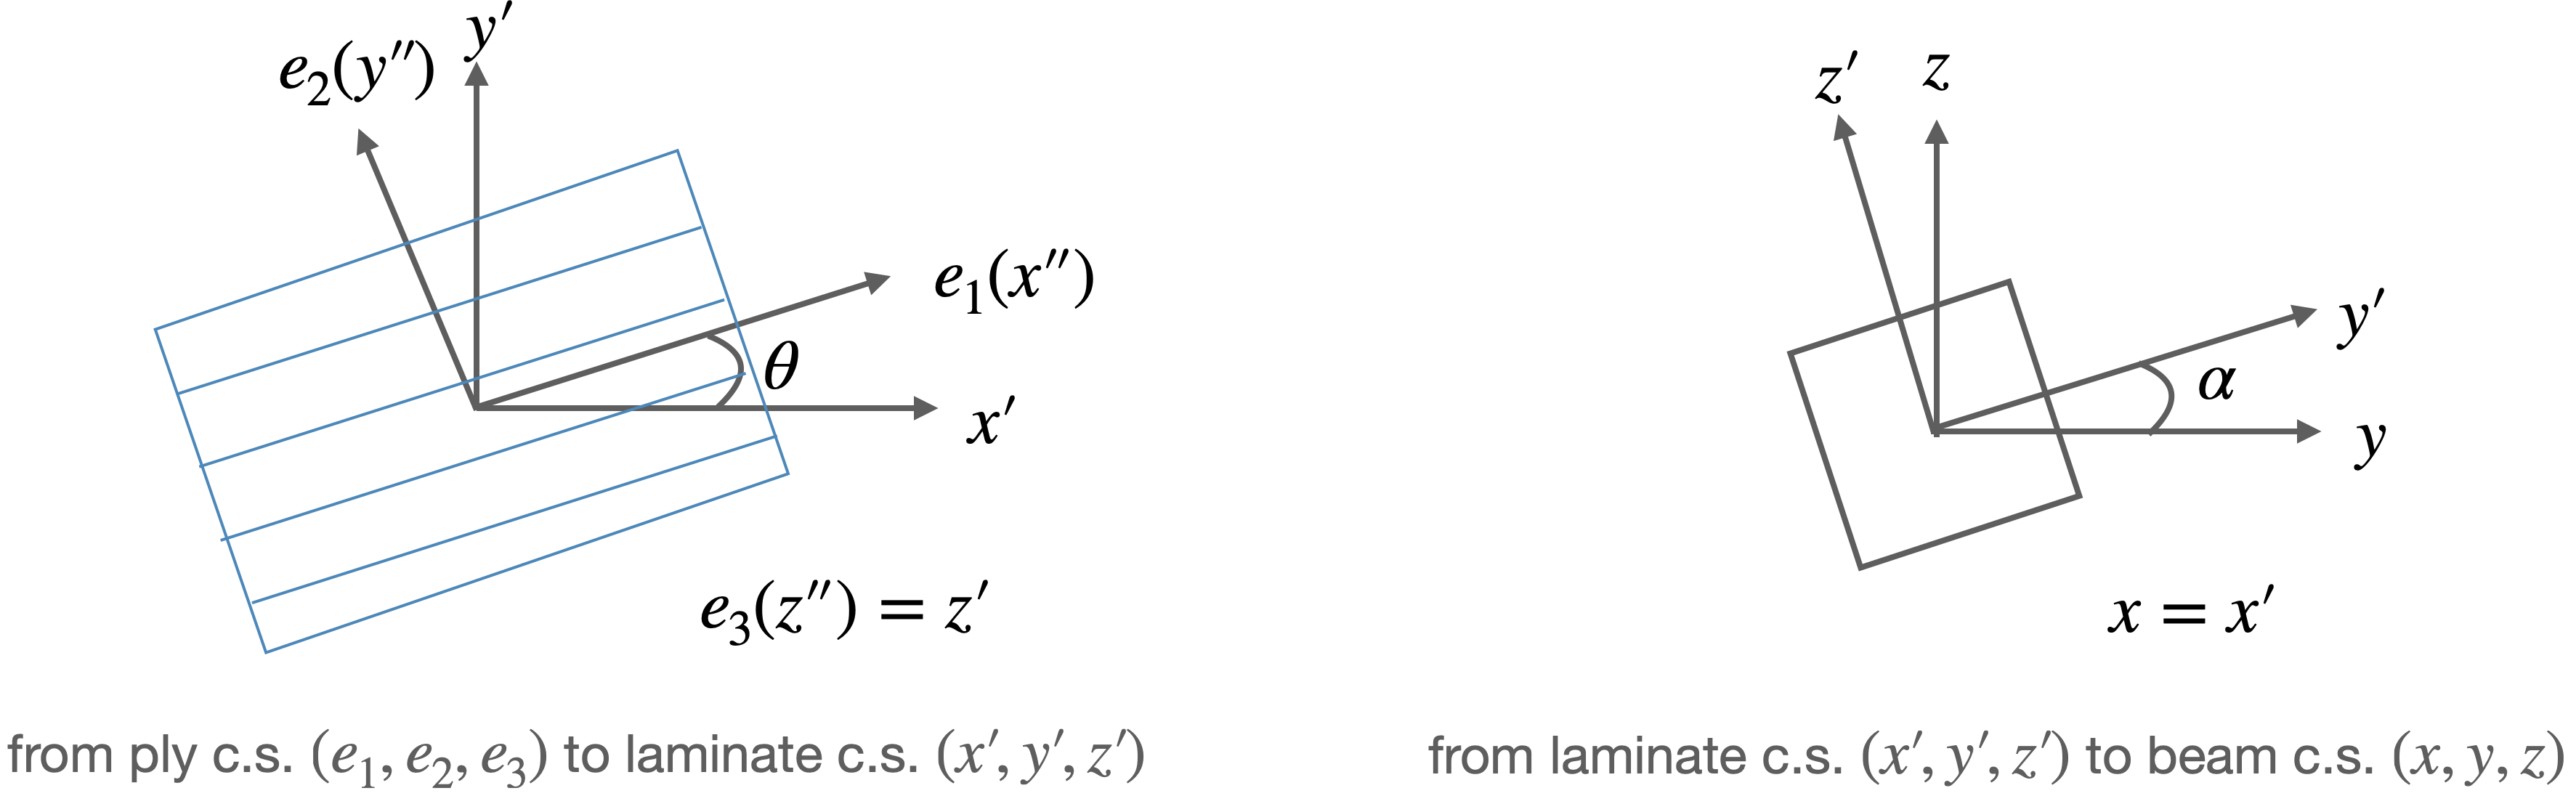
\includegraphics[width=4.0in]{cltcoordinates.png}
\caption{Coordinate system for classical lamiante theory.}
\label{fig:cltcoordinates}
\end{figure}

First, we assume that the thickness of the composite laminates (in the $e_3$ direction) is much smaller than its other two dimensions. In this case, we often make a plane stress assumption, which makes the problem two-dimensional.  This assumption means that:
\begin{equation}
\sigma_3 = \tau_{13} = \tau_{23} = 0
\end{equation}

For orthotropic materials, in plane stress, the constitutive
equations (\cref{eq:orthoconstit}) reduce to:
\begin{equation}
\left[
\begin{matrix}
\sigma_{1}\\
\sigma_{2}\\
0\\
\tau_{12}\\
0\\
0\\
\end{matrix}
\right]
=
\left[
\begin{matrix}
K_{11} & K_{12} & K_{13} & 0 & 0 & 0 \\
K_{21} & K_{22} & K_{23} & 0 & 0 & 0 \\
K_{31} & K_{32} & K_{33} & 0 & 0 & 0 \\
0 & 0 & 0 & K_{44} & 0 & 0 \\
0 & 0 & 0 & 0 & K_{55} & 0 \\
0 & 0 & 0 & 0 & 0 & K_{66}
\end{matrix}
\right]
\left[
\begin{matrix}
\epsilon_{1}\\
\epsilon_{2}\\
\epsilon_{3}\\
\gamma_{12}\\
\gamma_{13}\\
\gamma_{23}
\end{matrix}
\right]
\end{equation}
We immediately see that $\gamma_{13} = 0$ and $\gamma_{23} = 0$ and we can thus remove the associated rows and columns, and equations.
\begin{equation}
\left[
\begin{matrix}
\sigma_{1}\\
\sigma_{2}\\
0\\
\tau_{12}\\
\end{matrix}
\right]
=
\left[
\begin{matrix}
K_{11} & K_{12} & K_{13} & 0 \\
K_{21} & K_{22} & K_{23} & 0 \\
K_{31} & K_{32} & K_{33} & 0 \\
0 & 0 & 0 & K_{44} \\
\end{matrix}
\right]
\left[
\begin{matrix}
\epsilon_{1}\\
\epsilon_{2}\\
\epsilon_{3}\\
\gamma_{12}\\
\end{matrix}
\right]
\end{equation}

For the third equation:
\begin{equation}
    K_{31}\epsilon_1 + K_{32}\epsilon_2 + K_{33}\epsilon_3 = 0
\end{equation}
we can solve for $\epsilon_3$
\begin{equation}
    \epsilon_3 = -\frac{K_{31}}{K_{33}}\epsilon_1 - \frac{K_{32}}{K_{33}}\epsilon_2,
\end{equation}
then insert that into the first two equations to eliminate $\epsilon_3$.
\begin{equation}
\left[
\begin{matrix}
\sigma_{1}\\
\sigma_{2}\\
\tau_{12}\\
\end{matrix}
\right]
=
\left[
\begin{matrix}
K_{11} - \frac{K_{13}^2}{K_{33}} & K_{12} - \frac{K_{13}K_{23}}{K_{33}} & 0 \\
K_{12} - \frac{K_{23}K_{13}}{K_{33}} & K_{22} - \frac{K_{23}^2}{K_{33}} & 0 \\
0 & 0  & K_{44} \\
\end{matrix}
\right]
\left[
\begin{matrix}
\epsilon_{1}\\
\epsilon_{2}\\
\gamma_{12}\\
\end{matrix}
\right]
\end{equation}
For convenience, we define these grouping of stiffness constants with new names:
\begin{equation}
\left[
\begin{matrix}
\sigma_{1}\\
\sigma_{2}\\
\tau_{12}\\
\end{matrix}
\right]
=
\left[
\begin{matrix}
Q_{11} & Q_{12} & 0 \\
Q_{12} & Q_{22} & 0 \\
0 & 0  & Q_{33} \\
\end{matrix}
\right]
\left[
\begin{matrix}
\epsilon_{1}\\
\epsilon_{2}\\
\gamma_{12}\\
\end{matrix}
\right]
\end{equation}
where
\begin{equation}
Q_{11} = K_{11} - \frac{K_{13}^2}{K_{33}}
\end{equation}
\begin{equation}
Q_{12} = K_{12} - \frac{K_{13}K_{23}}{K_{33}}
\end{equation}
\begin{equation}
Q_{22} = K_{22} - \frac{K_{23}^2}{K_{33}}
\end{equation}
\begin{equation}
Q_{33} = K_{44}
\end{equation}

We can express these new stiffness properties in terms of the material properties.  Referring to \cref{eq:orthostiffness} we see that the reduced stiffness matrix is (removing the rows/columns of zeros, and ignoring all $\nu_{3i}$ contributions):
\begin{equation}
\left[
\begin{matrix}
\sigma_{1}\\
\sigma_{2}\\
\tau_{12}\\
\end{matrix}
\right]
=
\left[
\begin{matrix}
E_1 \Delta & E_1 \nu_{21} \Delta &  0 \\
E_2 \nu_{12} \Delta & E_2 \Delta & 0 \\
0 & 0 & G_{12} \\
\end{matrix}
\right]
\left[
\begin{matrix}
\epsilon_{1}\\
\epsilon_{2}\\
\gamma_{12}\\
\end{matrix}
\right]
\end{equation}
where
\begin{equation}
\Delta = \frac{1}{1 - \nu_{12}\nu_{21}}
\end{equation}
We can also derive this relationship directly by considering coupon tests where we alternate between a pure axial load in direction 1, a pure axial load in direction 2, and a pure shear test.

From this relationship we see that:
\begin{align}
Q_{11} &= \frac{E_1}{1 - \nu_{12}\nu_{21}}\\
Q_{22} &= \frac{E_2}{1 - \nu_{12}\nu_{21}}\\
Q_{12} &= \frac{\nu_{21}E_1}{1 - \nu_{12}\nu_{21}} = \frac{\nu_{12}E_2}{1 - \nu_{12}\nu_{21}}\\
Q_{33} &= G_{12}
\end{align}
These relationships apply to an orthotropic ply in plane stress.

These relationships apply in the principal orientation of the ply, but we often use plys at different angles. We derived coordinate transformations previously for the case with a coincident $z$-axis (\cref{eq:rotatezsigma,eq:rotatezeps}), though we now drop some of the rows/columns since we are in a plane stress state.
\begin{equation}
    T_\sigma =
\begin{bmatrix}
\cos^2\theta & \sin^2\theta &  -2 \sin\theta\cos\theta \\
\sin^2\theta & \cos^2\theta & 2 \sin\theta\cos\theta \\
\sin\theta\cos\theta & -\sin\theta\cos\theta & \cos^2\theta - \sin^2\theta \\
\end{bmatrix}
\end{equation}
and
\begin{equation}
    T_\epsilon =
\begin{bmatrix}
\cos^2\theta & \sin^2\theta &  -\sin\theta\cos\theta \\
\sin^2\theta & \cos^2\theta & \sin\theta\cos\theta \\
2 \sin\theta\cos\theta & -2 \sin\theta\cos\theta & \cos^2\theta - \sin^2\theta \\
\end{bmatrix}
\end{equation}
and the stiffness matrix is transformed as shown previously in \cref{eq:Ktrans}.

After rotation the stiffness matrix will typically be dense, though still symmetric, as shown in:
\begin{equation}
\left[
\begin{matrix}
\sigma_{x^\prime}\\
\sigma_{y^\prime}\\
\tau_{x^\prime y^\prime}\\
\end{matrix}
\right]
=
\left[
\begin{matrix}
Q_{x^\prime x^\prime } & Q_{x^\prime y^\prime} & Q_{x^\prime z^\prime } \\
Q_{x^\prime y^\prime} & Q_{y^\prime y^\prime} & Q_{y^\prime z^\prime } \\
Q_{x^\prime z^\prime } & Q_{y^\prime z^\prime}  & Q_{z^\prime z^\prime} \\
\end{matrix}
\right]
\left[
\begin{matrix}
\epsilon_{x^\prime}\\
\epsilon_{y^\prime}\\
\gamma_{x^\prime y^\prime}\\
\end{matrix}
\right]
\label{eq:KasQ}
\end{equation}
For notational simplicity, in the remainder of this section we use the indices 1, 2, 3, but should recall that we are really in the primed coordinate system.
\begin{equation}
\left[
\begin{matrix}
\sigma_{1}\\
\sigma_{2}\\
\tau_{12}\\
\end{matrix}
\right]
=
\left[
\begin{matrix}
Q_{11} & Q_{12} & Q_{13} \\
Q_{12} & Q_{22} & Q_{23} \\
Q_{13} & Q_{23}  & Q_{33} \\
\end{matrix}
\right]
\left[
\begin{matrix}
\epsilon_{1}\\
\epsilon_{2}\\
\gamma_{12}\\
\end{matrix}
\right]
\label{eq:KasQ}
\end{equation}


A ply is stacked on other plys, all with potentially different orientations and material properties, to form a laminate.  We can determine the resultant laminate forces and moments by integrating the various stresses across the thickness of the laminate.  We call the total height $h$ then the normal forces, per unit width, are given by:
\begin{equation}
N_1^\prime = \int_{-h/2}^{h/2} \sigma_1 dz
\label{eq:Nx}
\end{equation}
\begin{equation}
N_2^\prime = \int_{-h/2}^{h/2} \sigma_2 dz
\end{equation}
The resultant shear force on the laminate is:
\begin{equation}
V_{12}^\prime = \int_{-h/2}^{h/2} \tau_{12} dz
\end{equation}

The moments, per unit width, are given below where $z$ is measured starting from the midplane of the laminate.  Note that these definitions are not the typical mathematical definitions for moments, but rather are simply convenient definitions, which correspond to typical engineering definitions ($M_1$ is bending in the $x$-$z$ plane), but with the opposite sign of what is typically used.
\begin{equation}
M_1^\prime = \int_{-h/2}^{h/2} z \sigma_1 dz
\label{eq:M1}
\end{equation}
\begin{equation}
M_2^\prime = \int_{-h/2}^{h/2} z \sigma_2 dz
\end{equation}
the torque, which is produced equally about the $x$ and $y$ axes is:
\begin{equation}
T_{12}^\prime = \int_{-h/2}^{h/2} z \tau_{12} dz
\end{equation}

The average, or effective, stresses on the laminate can then be found by:
\begin{equation}
\bar\sigma_1 = \frac{1}{h} \int_{-h/2}^{h/2} \sigma_1 dz = \frac{N_1^\prime}{h}
\label{eq:effectivestress}
\end{equation}
Similarly,
\begin{equation}
\bar\sigma_2 = \frac{N_2^\prime}{h}
\end{equation}
\begin{equation}
\bar\tau_{12} = \frac{V_{12}^\prime}{h}
\end{equation}

% While properties vary from ply the ply, they are constant with a given ply, so the integration becomes a sum of integrals across each ply.
We will  drop the primes for convenience, for example, repeating \cref{eq:Nx}:
\begin{equation}
N_1 = \int_{-h/2}^{h/2} \sigma_1 dz
\end{equation}
But now introduce the stress relationship from the first equation in \cref{eq:KasQ}:
\begin{equation}
N_1 = \int_{-h/2}^{h/2} (Q_{11} \epsilon_1 + Q_{12} \epsilon_2 + Q_{13} \gamma_{12}) dz
\end{equation}

The stiffness properties are constant in each ply, but the strains may not be.  In the case of pure axial loading, they may be, but we may have coupling between axial and bending behavior.  Pure bending formulas ($\sigma = Mz/I$) are derived by assuming plane sections remain plane (see for example section 2.2 in my structures book), which means that the strain is linearly related to the curvature $\kappa$.  We continue using a convenient definition, which again differs by a negative sign from the typical engineering definition for curvature-strain relationship.  Thus, for pure bending we have:
\begin{equation}
\epsilon_1 = \kappa_1 z
\end{equation}
\begin{equation}
\epsilon_2 = \kappa_2 z
\end{equation}
\begin{equation}
\gamma_{12} = \kappa_{12} z
\end{equation}
In the general case, we expect to have coupling between these behaviors and so express the strain as a sum of a constant mid-plane strain, and a curvature component:
\begin{equation}
    \begin{aligned}
        \epsilon_1 &= \bar\epsilon_1 + \kappa_1 z \\
        \epsilon_2 &= \bar\epsilon_2 + \kappa_2 z \\
        \gamma_{12} &= \bar\gamma_{12} + \kappa_{12} z
    \end{aligned}
    \label{eq:straincurvature}
\end{equation}

We now substitute these expression into our equation:
\begin{equation}
N_1 = \int_{-h/2}^{h/2} (Q_{11} (\bar\epsilon_1 + \kappa_1 z) + Q_{12} (\bar\epsilon_2 + \kappa_2 z) + Q_{13} (\bar\gamma_{12} + \kappa_{12} z)) dz\\
\end{equation}
Since the midplane strains and curvatures are constant we pull them out of the integrals:
\begin{equation}
\begin{aligned}
N_1 =& \int_{-h/2}^{h/2} Q_{11} dz\, \bar\epsilon_1 + \int_{-h/2}^{h/2} Q_{12} dz\, \bar\epsilon_2 + \int_{-h/2}^{h/2} Q_{13} dz\, \bar\gamma_{12} \\ &+ \int_{-h/2}^{h/2} z Q_{11} dz\, \kappa_1 + \int_{-h/2}^{h/2} z Q_{12} dz\, \kappa_2 + \int_{-h/2}^{h/2} z Q_{13} dz\, \kappa_{12}
\end{aligned}
\end{equation}

We can now express this in matrix form, along with the other forces that follow the same form as:
\begin{equation}
\left[
\begin{matrix}
N_{1}\\
N_{2}\\
N_{12}\\
\end{matrix}
\right]
=
\left[
\begin{matrix}
A_{11} & A_{12} & A_{13} & B_{11} & B_{12} & B_{13} \\
A_{12} & A_{22} & A_{23} & B_{12} & B_{22} & B_{23} \\
A_{13} & A_{23} & A_{33} & B_{13} & B_{23} & B_{33} \\
\end{matrix}
\right]
\left[
\begin{matrix}
\bar\epsilon_{1}\\
\bar\epsilon_{2}\\
\bar\gamma_{12}\\
\kappa_1 \\
\kappa_2 \\
\kappa_{12} \\
\end{matrix}
\right]
\end{equation}
where
\begin{equation}
A_{ij} = \int_{-h/2}^{h/2} Q_{ij} dz
\end{equation}
and
\begin{equation}
B_{ij} = \int_{-h/2}^{h/2} z Q_{ij} dz
\end{equation}

For our case, the stiffness $Q$ is constant in a given ply, so the integral simplifies to a summation across all $k$ plys in the laminate:
\begin{equation}
A_{ij} = \sum_{k=1}^n Q_{ij} (z_k - z_{k-1})
\end{equation}
and
\begin{equation}
B_{ij} = \sum_{k=1}^n Q_{ij} \frac{(z_k^2 - z_{k-1}^2)}{2}
\end{equation}
Again, recall that $z$ is measured from the center plane of the laminate.


We follow the same process, where we write out \cref{eq:M1}, again dropping the prime for convenience:
\begin{equation}
M_1 = \int_{-h/2}^{h/2} z \sigma_1 dz
\end{equation}
then expand out the stress term from \cref{eq:KasQ}:
\begin{equation}
M_1 = \int_{-h/2}^{h/2} (z Q_{11} \epsilon_1 + z Q_{22} \epsilon_2 + z Q_{13} \gamma_{12}) dz
\end{equation}
Substituting in the expressions for strain (\cref{eq:straincurvature}):
\begin{equation}
M_1 = \int_{-h/2}^{h/2} (Q_{11} (z \bar\epsilon_{1} + z^2 \kappa_1) + Q_{22} (z \bar\epsilon_{2} + z^2 \kappa_2) +  Q_{13} (z \bar\gamma_{12} + z^2 \kappa_{12})) dz
\end{equation}
We now change the integration to a summation across each ply (since $Q$ and $\kappa$ are constant in each ply).  We see that the linear terms, will result in the same expressions for $B$.
\begin{equation}
\left[
\begin{matrix}
M_{1}\\
M_{2}\\
M_{12}\\
\end{matrix}
\right]
=
\left[
\begin{matrix}
    B_{11} & B_{12} & B_{13} & D_{11} & D_{12} & D_{13} \\
    B_{12} & B_{22} & B_{23}  & D_{12} & D_{22} & D_{23} \\
    B_{13} & B_{23} & B_{33} & D_{13} & D_{23} & D_{33} \\
\end{matrix}
\right]
\left[
\begin{matrix}
\bar\epsilon_{1}\\
\bar\epsilon_{2}\\
\bar\gamma_{12}\\
\kappa_1 \\
\kappa_2 \\
\kappa_{12} \\
\end{matrix}
\right]
\end{equation}
where
\begin{equation}
D_{ij} = \sum_{k=1}^n Q_{ij} \frac{(z_k^3 - z_{k-1}^3)}{3}
\end{equation}

Stacking both sets of equations together results in:
\begin{equation}
    \left[
    \begin{matrix}
    N_{1}\\
    N_{2}\\
    N_{12}\\
    M_{1}\\
    M_{2}\\
    M_{12}\\
    \end{matrix}
    \right]
    =
    \left[
    \begin{matrix}
        A_{11} & A_{12} & A_{13} & B_{11} & B_{12} & B_{13} \\
        A_{12} & A_{22} & A_{23} & B_{12} & B_{22} & B_{23} \\
        A_{13} & A_{23} & A_{33} & B_{13} & B_{23} & B_{33} \\
        B_{11} & B_{12} & B_{13} & D_{11} & D_{12} & D_{13} \\
        B_{12} & B_{22} & B_{23}  & D_{12} & D_{22} & D_{23} \\
        B_{13} & B_{23} & B_{33} & D_{13} & D_{23} & D_{33} \\
    \end{matrix}
    \right]
    \left[
    \begin{matrix}
    \bar\epsilon_{1}\\
    \bar\epsilon_{2}\\
    \bar\gamma_{12}\\
    \kappa_1 \\
    \kappa_2 \\
    \kappa_{12} \\
    \end{matrix}
    \right]
    \label{eq:ABD}
    \end{equation}
    Note that since the expression for $B$ is even (squared terms), then $B = 0$ for symmetric laminates.  The expression for $A$ is just a stiffness multiplied by the thickness of the ply, so the ordering of the plys does not change $A$. That provides a design degree of freedom.  If the laminate is balanced (which means for every ply at $+\theta$ there is the same ply at $-\theta$ somewhere in the laminate) then $A_{13} = A_{23} = D_{13} = D_{23} = 0$.  This occurs because the two corresponding values for $Q$ will be the same, but with opposite signs ($Q_{13}$ and $Q_{23}$ only arise from rotation, and the properties will be the same, just rotated in different directions with different signs), and the ordering does not matter for the entries in $A$ as already discussed.


While the above equation was expressed to compute forces and moments as a function of strains and curvatures, we generally would like this relationship inverted since it is typically the forces and moments that are known. The matrix inversion can be computed as follows using a block diagonal representation for \cref{eq:ABD}:
\begin{align}
N &= A \epsilon + B \kappa \\
M &= B \epsilon + D \kappa  \label{eq:Msecond}
\end{align}
We solve the first equation for $\epsilon$:
\begin{equation}
\begin{aligned}
\epsilon &= A^{-1}(N - B \kappa)\\
 &= A^{-1}N - A^{-1} B \kappa \label{eq:esecond}
\end{aligned}
\end{equation}
We now plug this result into \cref{eq:Msecond}:
\begin{equation}
\begin{aligned}
M &= B A^{-1}N - B A^{-1} B \kappa + D \kappa\\
 &= B A^{-1} N + (D - B A^{-1} B) \kappa
\end{aligned}
\end{equation}
We now solve this expression for $\kappa$:
\begin{equation}
\begin{aligned}
\kappa &= (D - B A^{-1} B)^{-1} (M - B A^{-1} N )\\
 &= (D - B A^{-1} B)^{-1} M - (D - B A^{-1} B)^{-1} B A^{-1} N \label{eq:kdone}
\end{aligned}
\end{equation}
Finally, we plug this into \cref{eq:esecond}
\begin{equation}
\begin{aligned}
\epsilon &= A^{-1}N - A^{-1} B \left[(D - B A^{-1} B)^{-1} M - (D - B A^{-1} B)^{-1} B A^{-1} N \right] \\
&= (A^{-1} + A^{-1} B (D - B A^{-1} B)^{-1} B A^{-1} ) N - A^{-1} B (D - B A^{-1} B)^{-1} M \label{eq:epsdone}
\end{aligned}
\end{equation}
The results \cref{eq:epsdone,eq:kdone} we can write as:
\begin{align}
\epsilon &= \alpha N + \beta M \\
\kappa &= \beta_2 N + \delta M
\end{align}
where
\begin{align}
\alpha &= A^{-1} + A^{-1} B [D - B A^{-1} B]^{-1} B A^{-1}\\
\beta &= - A^{-1} B [D - B A^{-1} B]^{-1}\\
\beta_2 &= - [D - B A^{-1} B]^{-1} B A^{-1}\\
\delta &= [D - B A^{-1} B]^{-1}
\end{align}
We used the subscript two because we know that $\beta_2$ should be the transpose of $\beta$ as the original overall stiffness matrix was symmetric so the overall compliance matrix must also be symmetric (although note that $\beta$ itself is not necessarily symmetric).  We can show that this is the case:
\begin{equation}
\beta^T = - [D - B A^{-1} B]^{-T} B^T A^{-T} \\
\end{equation}
But since $A, B$, and $D$ are all symmetric, and $B A^{-1} B$ is symmetric ($(B A^{-1} B)^T = B^T A^{-T} B^T = B A^{-1} B$), and the sum of symmetric matrices is symmetric then the above simplifies to:
\begin{equation}
\begin{aligned}
\beta^T &= - [D - B A^{-1} B]^{-1} B A^{-1} \\
&= \beta_2
\end{aligned}
\end{equation}
Thus, in block diagonal form we have:
\begin{equation}
\begin{bmatrix}
    \epsilon\\
    \kappa
\end{bmatrix}
=
\begin{bmatrix}
    \alpha & \beta \\
    \beta^T & \delta
\end{bmatrix}
\begin{bmatrix}
    N\\
    M
\end{bmatrix}
\end{equation}
Or more explicitly as:
\begin{equation}
\left[
\begin{matrix}
\bar\epsilon_{1}\\
\bar\epsilon_{2}\\
\bar\gamma_{12}\\
\kappa_1 \\
\kappa_2 \\
\kappa_{12} \\
\end{matrix}
\right]
=
\left[
\begin{matrix}
    \alpha_{11} & \alpha_{12} & \alpha_{13} & \beta_{11} & \beta_{12} & \beta_{13} \\
    \alpha_{12} & \alpha_{22} & \alpha_{23} & \beta_{21} & \beta_{22} & \beta_{23} \\
    \alpha_{13} & \alpha_{23} & \alpha_{33} & \beta_{31} & \beta_{32} & \beta_{33} \\
    \beta_{11} & \beta_{21} & \beta_{31} & \delta_{11} & \delta_{12} & \delta_{13} \\
    \beta_{12} & \beta_{22} & \beta_{32}  & \delta_{12} & \delta_{22} & \delta_{23} \\
    \beta_{13} & \beta_{23} & \beta_{33} & \delta_{13} & \delta_{23} & \delta_{33} \\
\end{matrix}
\right]
\left[
\begin{matrix}
N_{1}\\
N_{2}\\
N_{12}\\
M_{1}\\
M_{2}\\
M_{12}\\
\end{matrix}
\right]
\label{eq:ADBinverse}
\end{equation}

% with
% \begin{align}
% \alpha &= A^{-1} + A^{-1}B[D - B A^{-1} B]^{-1} B A^{-1}\\
% \beta &= -A B[D - BA^{-1} B]^{-1} \\
% \delta &= [D - BA^{-1} B]^{-1}
% \end{align}
% Note that $\beta$ is not necessarily symmetric and that the lower left matrix is the transpose of the upper right matrix.

For a symmetric laminate, a common scenario, $B = 0$ as discussed previously, and the above equations simplify greatly to:
\begin{align}
\alpha &= A^{-1} \\
\beta &= 0 \\
\delta &= D^{-1}
\end{align}
These inverses are often given a shorthand in this case:
\begin{align}
\alpha &= A^{-1} = a\\
\beta &= 0 \\
\delta &= D^{-1} = d
\end{align}

Now that we have ``stiffness and compliance'' relationships we can determine effective elastic constants for the laminate as a whole. First, let's consider a case with uniaxial loading ($N_1 \ne 0$, but all other loads at zero).  From the first two equations of \cref{eq:ADBinverse} we see that:
\begin{align}
\bar\epsilon_1 &= \alpha_{11} N_1 \label{eq:reduce1}\\
\bar\epsilon_2 &= \alpha_{12} N_1 \label{eq:reduce2}
\end{align}
Recall that the average laminate stress is related to the normal force as shown in \cref{eq:effectivestress}.
\begin{equation}
\bar\epsilon_1 = \alpha_{11} \bar\sigma_1 h
\end{equation}
or
\begin{equation}
    \bar\sigma_1 = \frac{1}{\alpha_{11} h} \bar\epsilon_1 \\
\end{equation}
Since, the definition of the effective axial stiffness is:
\begin{equation}
    \bar\sigma_1 = E_{1a} \bar\epsilon_1 \\
\end{equation}
then:
\begin{equation}
E_{1a} = \frac{1}{\alpha_{11} h}
\end{equation}
The same analysis occurs for pure axial loading in the other direction, as well as a pure shear stress relating a shear strain.

Combining \cref{eq:reduce1,eq:reduce2} we can determine an expression for Poisson's ratio.  We see that:
\begin{equation}
    \bar\epsilon_2 = \frac{\alpha_{12}}{\alpha_{11}} \bar\epsilon_1
\end{equation}
From the definition of Poisson's ratio:
\begin{equation}
    \bar\epsilon_2 = -\nu_{12} \bar\epsilon_1
\end{equation}
we see that:
\begin{equation}
    \nu_{12} = -\frac{\alpha_{12}}{\alpha_{11}}
\end{equation}
The same approach with loading in the other direction will allow us to find $\nu_{21}$.

Finally, let's consider a pure moment ($M_1 \ne 0$, all other loads zero).  The fourth equation tells us that:
\begin{equation}
\kappa_1 = \delta_{11} M_1
\end{equation}
Recall that $M_1$ is really the moment per unit width ($M_1^\prime$, see \cref{eq:M1}), so in terms of the effective laminate moment would be:
\begin{equation}
\kappa_1 = \delta_{11} \frac{M_1}{w}
\end{equation}
From any structures text we see that a pure moment is related to curvature as follows:
\begin{equation}
M_1 = E \kappa_1 I_1
\end{equation}
where $I_1$ for a rectangular section would be $I_1 = w h^3/12$.  Putting those together and rearranging results in:
\begin{equation}
\kappa_1 = M_1 \frac{12}{E w h^3}
\end{equation}
Comparing these two equations shows that
\begin{equation}
     \frac{\delta_{11}}{w} = \frac{12}{E w h^3}
\end{equation}
so the effective bending momentum of elasticity is:
\begin{equation}
E_{1b} = \frac{12}{\delta_{11} h^3}
\end{equation}
Note that the modulus of elasticity predicted by pure axial loading and by pure bending are likely different, and for a combined load case the more conservative is likely used.  The remaining constants workout in the same way.  In summary we have:
\begin{align}
    \bar E_{1a} &= \frac{1}{h \alpha_{11}}\\
    \bar E_{2a} &= \frac{1}{h \alpha_{22}}\\
    \bar G_{12a} &= \frac{1}{h \alpha_{33}}\\
    \nu_{12a} &= -\alpha_{12}/\alpha_{11}\\
    \nu_{21a} &= -\alpha_{12}/\alpha_{22}\\
    \bar E_{1b} &= \frac{12}{h^3 \delta_{11}}\\
    \bar E_{2b} &= \frac{12}{h^3 \delta_{22}}\\
    \bar G_{12b} &= \frac{12}{h^3 \delta_{33}}\\
    \nu_{12b} &= -\delta_{12}/\delta_{11}\\
    \nu_{21b} &= -\delta_{12}/\delta_{22}
\end{align}


With the midplane strains and curvature computed through (\cref{eq:ADBinverse}), we can compute strain through the laminate (\cref{eq:straincurvature}), which we express in vector form:
\begin{equation}
\epsilon^\prime_i(z) = \bar\epsilon_i + \kappa_i z
\end{equation}
With the strains in the laminate coordinate system we can compute the stresses across the laminate using \cref{eq:KasQ}.
\begin{equation}
\sigma^\prime_i(z) = \bar{Q} \epsilon^\prime_i(z)
\end{equation}
Finally, we can rotate the stresses back to the ply orientations (see \cref{eq:stressmapping} where we are now going from the primed coordinate system back to the ply---double primed---coordinate system):
\begin{align}
\sigma^{\prime\prime} &= T_\sigma^{-1} \sigma^\prime\\
 &= T_\epsilon^T \sigma^\prime
\end{align}
and
\begin{align}
\epsilon^{\prime\prime} &= T_\epsilon^{-1} \epsilon^\prime\\
    &= T_\sigma^T \epsilon^\prime
\end{align}

Once we have laminate properties, we now need to integrate to obtain beam-level properties.  To accomplish this we use the methodology summarized by Koll\'{a}r and Springer, which we do not repeat here \cite{Kollar2003}.

In that method we get strains and streses in the laminate orientation and need to rotate to the beam orientation (from primed to unprimed in right-side of \cref{fig:cltcoordinates}).  The transformation is:
\begin{equation}
\begin{aligned}
    x &= x^\prime \\
    y &= y^\prime \cos\alpha - z^\prime \sin\alpha\\
    z &= y^\prime \sin\alpha + z^\prime \cos\alpha
\end{aligned}
\end{equation}
The associated rotation matrix is then (using \cref{eq:Rmatrix}):
\begin{equation}
    R =
    \begin{bmatrix}
        1 & 0 & 0 \\
        0 & \cos\alpha & -\sin\alpha \\
        0 & \sin\alpha & \cos\alpha \\
    \end{bmatrix}
    \end{equation}
The transformation matrix $T_\sigma$ is:
\begin{equation}
    T_\sigma^{(2)} =
\begin{bmatrix}
1 & 0 & 0 & 0 & 0 & 0 \\
0 & \cos^2\theta & \sin^2\theta & 0 &  0  & -2\sin\alpha\cos\alpha  \\
0 &  \sin^2\theta  &  \cos^2\theta  & 0  &  0   &   2\sin\alpha\cos\alpha   \\
0 & 0 & 0 & \cos\alpha & -\sin\alpha & 0 \\
0 & 0 & 0 & \sin\alpha & \cos\alpha & 0 \\
0 & \sin\alpha\cos\alpha & -\sin\alpha\cos\alpha  & 0 & 0 & \cos^2\alpha - \sin^2\alpha \\
\end{bmatrix}
\end{equation}
and
\begin{equation}
    T_\epsilon^{(2)} =
\begin{bmatrix}
1 & 0 & 0 & 0 & 0 & 0 \\
0 & \cos^2\theta & \sin^2\theta & 0 &  0  & -\sin\alpha\cos\alpha  \\
0 &  \sin^2\theta  &  \cos^2\theta  & 0  &  0   &   \sin\alpha\cos\alpha   \\
0 & 0 & 0 & \cos\alpha & -\sin\alpha & 0 \\
0 & 0 & 0 & \sin\alpha & \cos\alpha & 0 \\
0 & 2\sin\alpha\cos\alpha & -2\sin\alpha\cos\alpha  & 0 & 0 & \cos^2\alpha - \sin^2\alpha \\
\end{bmatrix}
\end{equation}

Finally, we transform from primed to unprimed coordinate systems:
\begin{align}
\sigma &= T_\sigma^{(2)} \sigma^\prime\\
\epsilon &= T_\epsilon^{(2)} \epsilon^\prime
\end{align}

\section{Finite Element Approach for Section Properties}

This method of the previous section assumes thin sections, and the beam model does not always accurately compute some of the coupling behavior and transverse loading. In this section we use a more general finite element approach that can capture these behaviors, with a tradeoff in computational cost.

We reorder the stresses and strains the match that used by other theory documents that will be discussed later (note that these are mapped back later to match the ordering for GXBeam):
\begin{equation}
\sigma = [\sigma_x, \sigma_y, \sigma_{xy}, \sigma_{xz}, \sigma_{yz}, \sigma_{z}]
\label{eq:sigmareorder}
\end{equation}
\begin{equation}
\epsilon = [\epsilon_x, \epsilon_y, \epsilon_{xy}, \epsilon_{xz}, \epsilon_{yz}, \epsilon_{z}]
\end{equation}
where $z$ is the axial direction.

We then need to reorder the stiffness matrix in \cref{eq:orthostiffness} as follows.  Note that the matrix is symmetric. In \cref{eq:orthostiffness} it wasn't explicitly written that way, but using \cref{eq:nue} we can see that is.  Below we explicitly write it as symmetric.
\begin{equation}
K
=
\left[
\begin{matrix}
E_2(1 - \nu_{13}\nu_{31})\Delta & E_2(\nu_{32} + \nu_{12}\nu_{31})\Delta & 0 & 0 & 0 & E_1(\nu_{21} + \nu_{31}\nu_{23})\Delta \\
E_2(\nu_{32} + \nu_{12}\nu_{31})\Delta & E_3(1 - \nu_{12}\nu_{21})\Delta & 0 & 0 & 0 & E_1(\nu_{31} + \nu_{21}\nu_{32})\Delta \\
0 & 0 & G_{23} & 0 & 0 & 0 \\
0 & 0 & 0 & G_{12} & 0 & 0 \\
0 & 0 & 0 & 0 & G_{13} & 0 \\
E_1(\nu_{21} + \nu_{31}\nu_{23})\Delta & E_1(\nu_{31} + \nu_{21}\nu_{32})\Delta & 0 & 0 & 0 & E_1(1 - \nu_{23}\nu_{32})\Delta \\
\end{matrix}
\right]
\end{equation}

The stiffness matrix given in the ply frame must now be converted to the element frame, and then from the element frame to the global frame.  These coordinate systems are shown in \cref{fig:cs}.  For convenience we refer to the ply frame both with the $1, 2, 3$ indices, as well as the $x^{\prime\prime}, y^{\prime\prime}, z^{\prime\prime}$ indices (the former is used for specifying the material properties, whereas the latter is clearer in the rotations).

\begin{figure}[htbp]
\centering
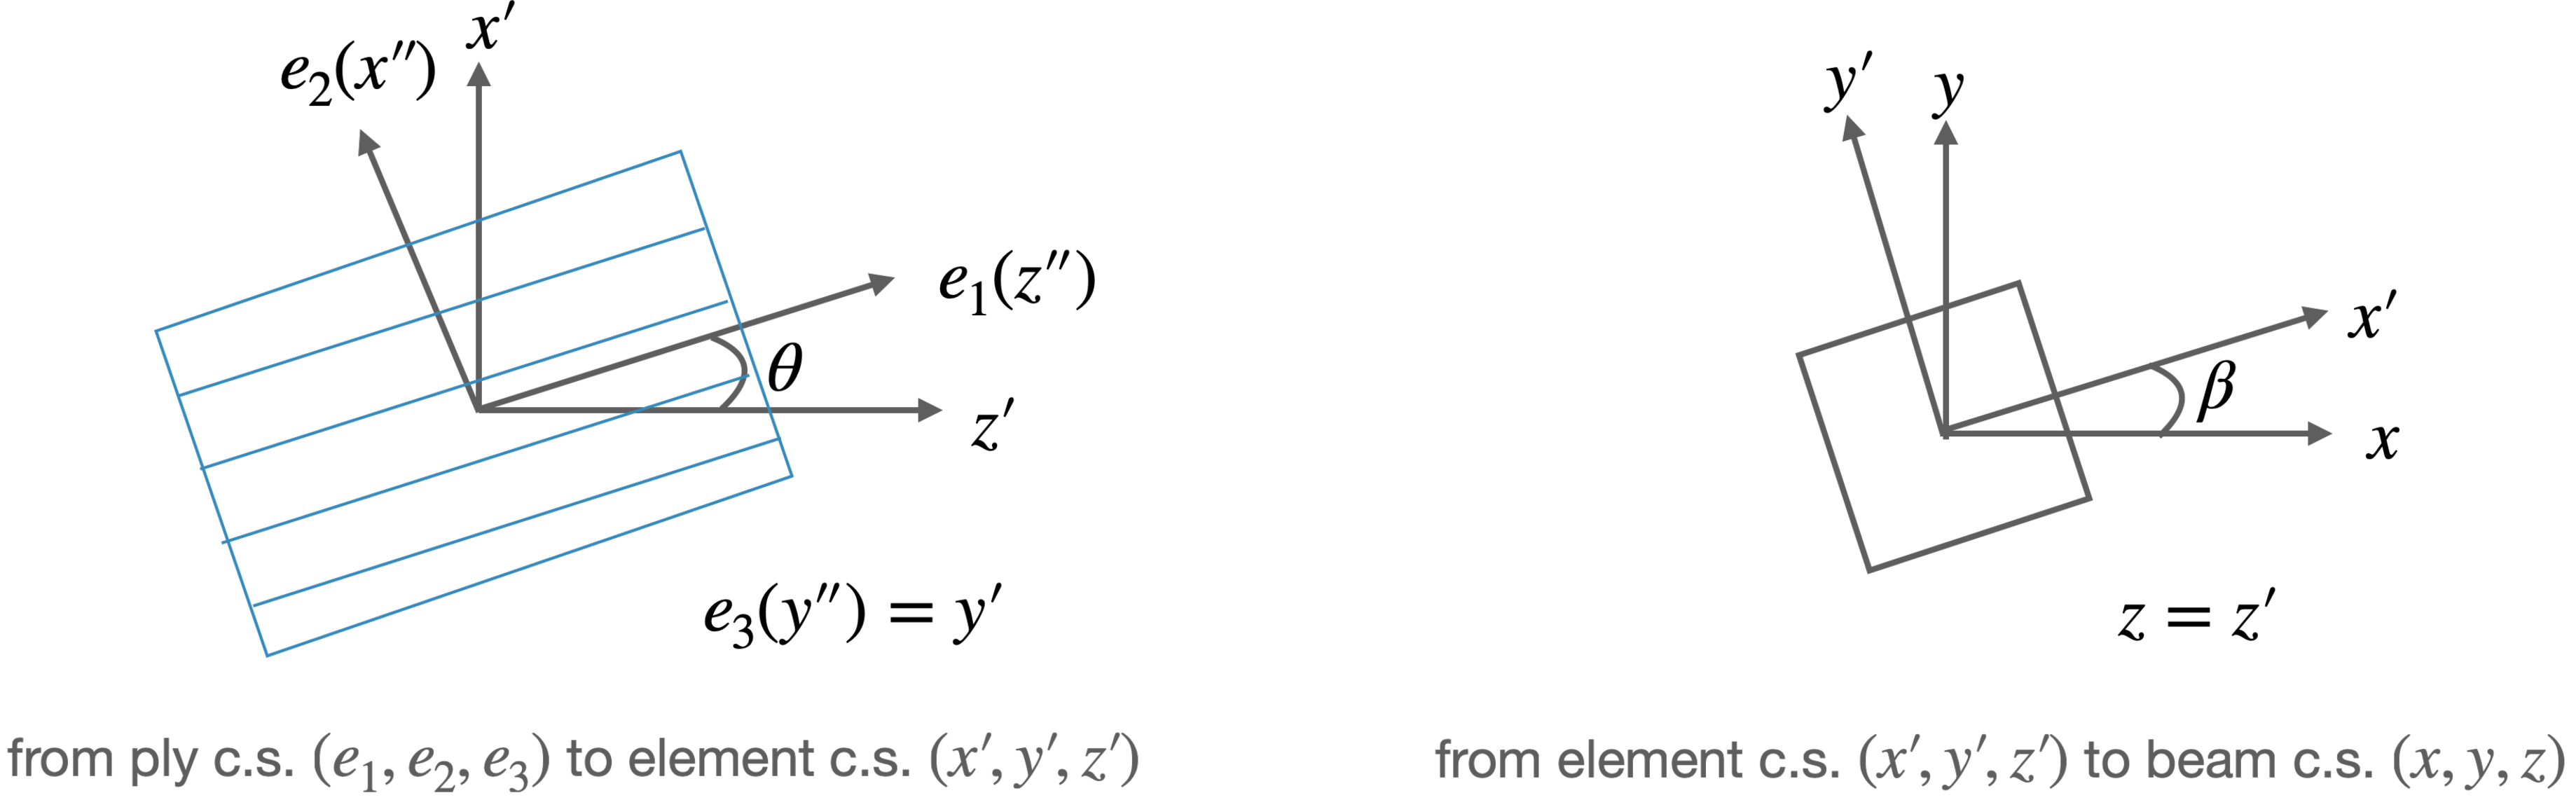
\includegraphics[width=4.5in]{cs}
\caption{Coordinate systems used in this analysis.}
\label{fig:cs}
\end{figure}

For the first rotation we see that:
\begin{equation}
\begin{aligned}
    x^\prime &= x^{\prime\prime} \cos\theta + z^{\prime\prime} \sin\theta\\
    y^\prime &= y^{\prime\prime}\\
    z^\prime &= -x^{\prime\prime} \sin\theta + z^{\prime\prime} \cos\theta
\end{aligned}
\end{equation}
Thus, the rotation matrix (\cref{eq:Rmatrix}) is:
\begin{equation}
R_\theta = \begin{bmatrix}
\cos\theta & 0 & \sin\theta \\
0 & 1 & 0 \\
-\sin\theta & 0 & \cos\theta \\
\end{bmatrix}
\end{equation}

We can now create the transformation matrix $T_\sigma$ (\cref{eq:Tsigma}) except that the above derivation used a different ordering of the stresses.  Using the ordering of this section (\cref{eq:sigmareorder}) we have:
\begin{equation}
T_\sigma = \begin{bmatrix}
R_{11}^2 & R_{12}^2  & 2 R_{11}R_{12} & 2 R_{11}R_{13} & 2 R_{12}R_{13} & R_{13}^2 \\
R_{21}^2 & R_{22}^2  & 2 R_{21}R_{22} & 2 R_{21}R_{23} & 2 R_{22}R_{23} & R_{23}^2\\
R_{11}R_{21} & R_{12}R_{22}  & R_{11}R_{22} + R_{12}R_{21} & R_{11}R_{23} + R_{13}R_{21} & R_{12}R_{23} + R_{13}R_{22} & R_{13}R_{23}\\
R_{11}R_{31} & R_{12}R_{32}  & R_{11}R_{32} + R_{12}R_{31} & R_{11}R_{33} + R_{13}R_{31} & R_{12}R_{33} + R_{13}R_{32} & R_{13}R_{33}\\
R_{21}R_{31} & R_{22}R_{32}  & R_{21}R_{32} + R_{22}R_{31} & R_{21}R_{33} + R_{23}R_{31} & R_{22}R_{33} + R_{23}R_{32} & R_{23}R_{33}\\
R_{31}^2 & R_{32}^2  & 2 R_{31}R_{32} & 2 R_{31}R_{33} & 2 R_{32}R_{33} & R_{33}^2\\
\end{bmatrix}
\end{equation}

Applying our specific rotation matrix $R_\theta$ to this case gives the first transformation:
\begin{equation}
{T_\sigma}_\theta =
\begin{bmatrix}
\cos^2\theta & 0 & 0 & 2 \cos\theta \sin\theta & 0 & \sin^2\theta \\
0 & 1 & 0 & 0 & 0 & 0 \\
0 & 0 & \cos\theta & 0 & \sin\theta & 0 \\
-\sin\theta\cos\theta & 0 & 0 & \cos^2\theta-\sin^2\theta & 0 & \cos\theta \sin\theta \\
0 & 0 & -\sin\theta & 0 & \cos\theta & 0 \\
\sin^2\theta & 0 & 0 & -2\sin\theta\cos\theta & 0 & \cos^2\theta \\
\end{bmatrix}
\end{equation}
We then use the transformation in  \cref{eq:Ktrans} to transform the stiffness matrix to the element coordinate system.

We repeat this process for the second transformation. Referring to the right hand side of \cref{fig:cs} we see that:
\begin{equation}
\begin{aligned}
    x &= x^\prime \cos\beta - y^\prime \sin\beta\\
    y &= x^\prime \sin\beta + y^\prime \cos\beta\\
    z &= z^\prime
\end{aligned}
\end{equation}
Thus:
\begin{equation}
R_\beta = \begin{bmatrix}
\cos\beta & -\sin\beta & 0 \\
\sin\beta & \cos\beta & 0 \\
0 & 0 & 1\\
\end{bmatrix}
\end{equation}
The resulting transformation matrix is then:
\begin{equation}
{T_\sigma}_\beta =
\begin{bmatrix}
    \cos^2\beta & \sin^2\beta & -2\sin\beta\cos\beta & 0 & 0 & 0 \\
    \sin^2\beta & \cos^2\beta & 2 \cos\beta \sin\beta & 0 & 0 & 0 \\
\sin\beta\cos\beta & -\cos\beta \sin\beta & \cos^2\beta-\sin^2\beta & 0 & 0 & 0 \\
0 & 0 & 0 & \cos\beta & -\sin\beta & 0 \\
0 & 0 & 0 & \sin\beta & \cos\beta & 0 \\
0 & 0 & 0 & 0 & 0 & 1 \\
\end{bmatrix}
\end{equation}

While $\theta$ (ply angle) must be a user input, $\beta$ we can compute from the geometry.
The nodes in an element are defined in the order shown in \cref{fig:element}.
\begin{figure}[htbp]
\centering
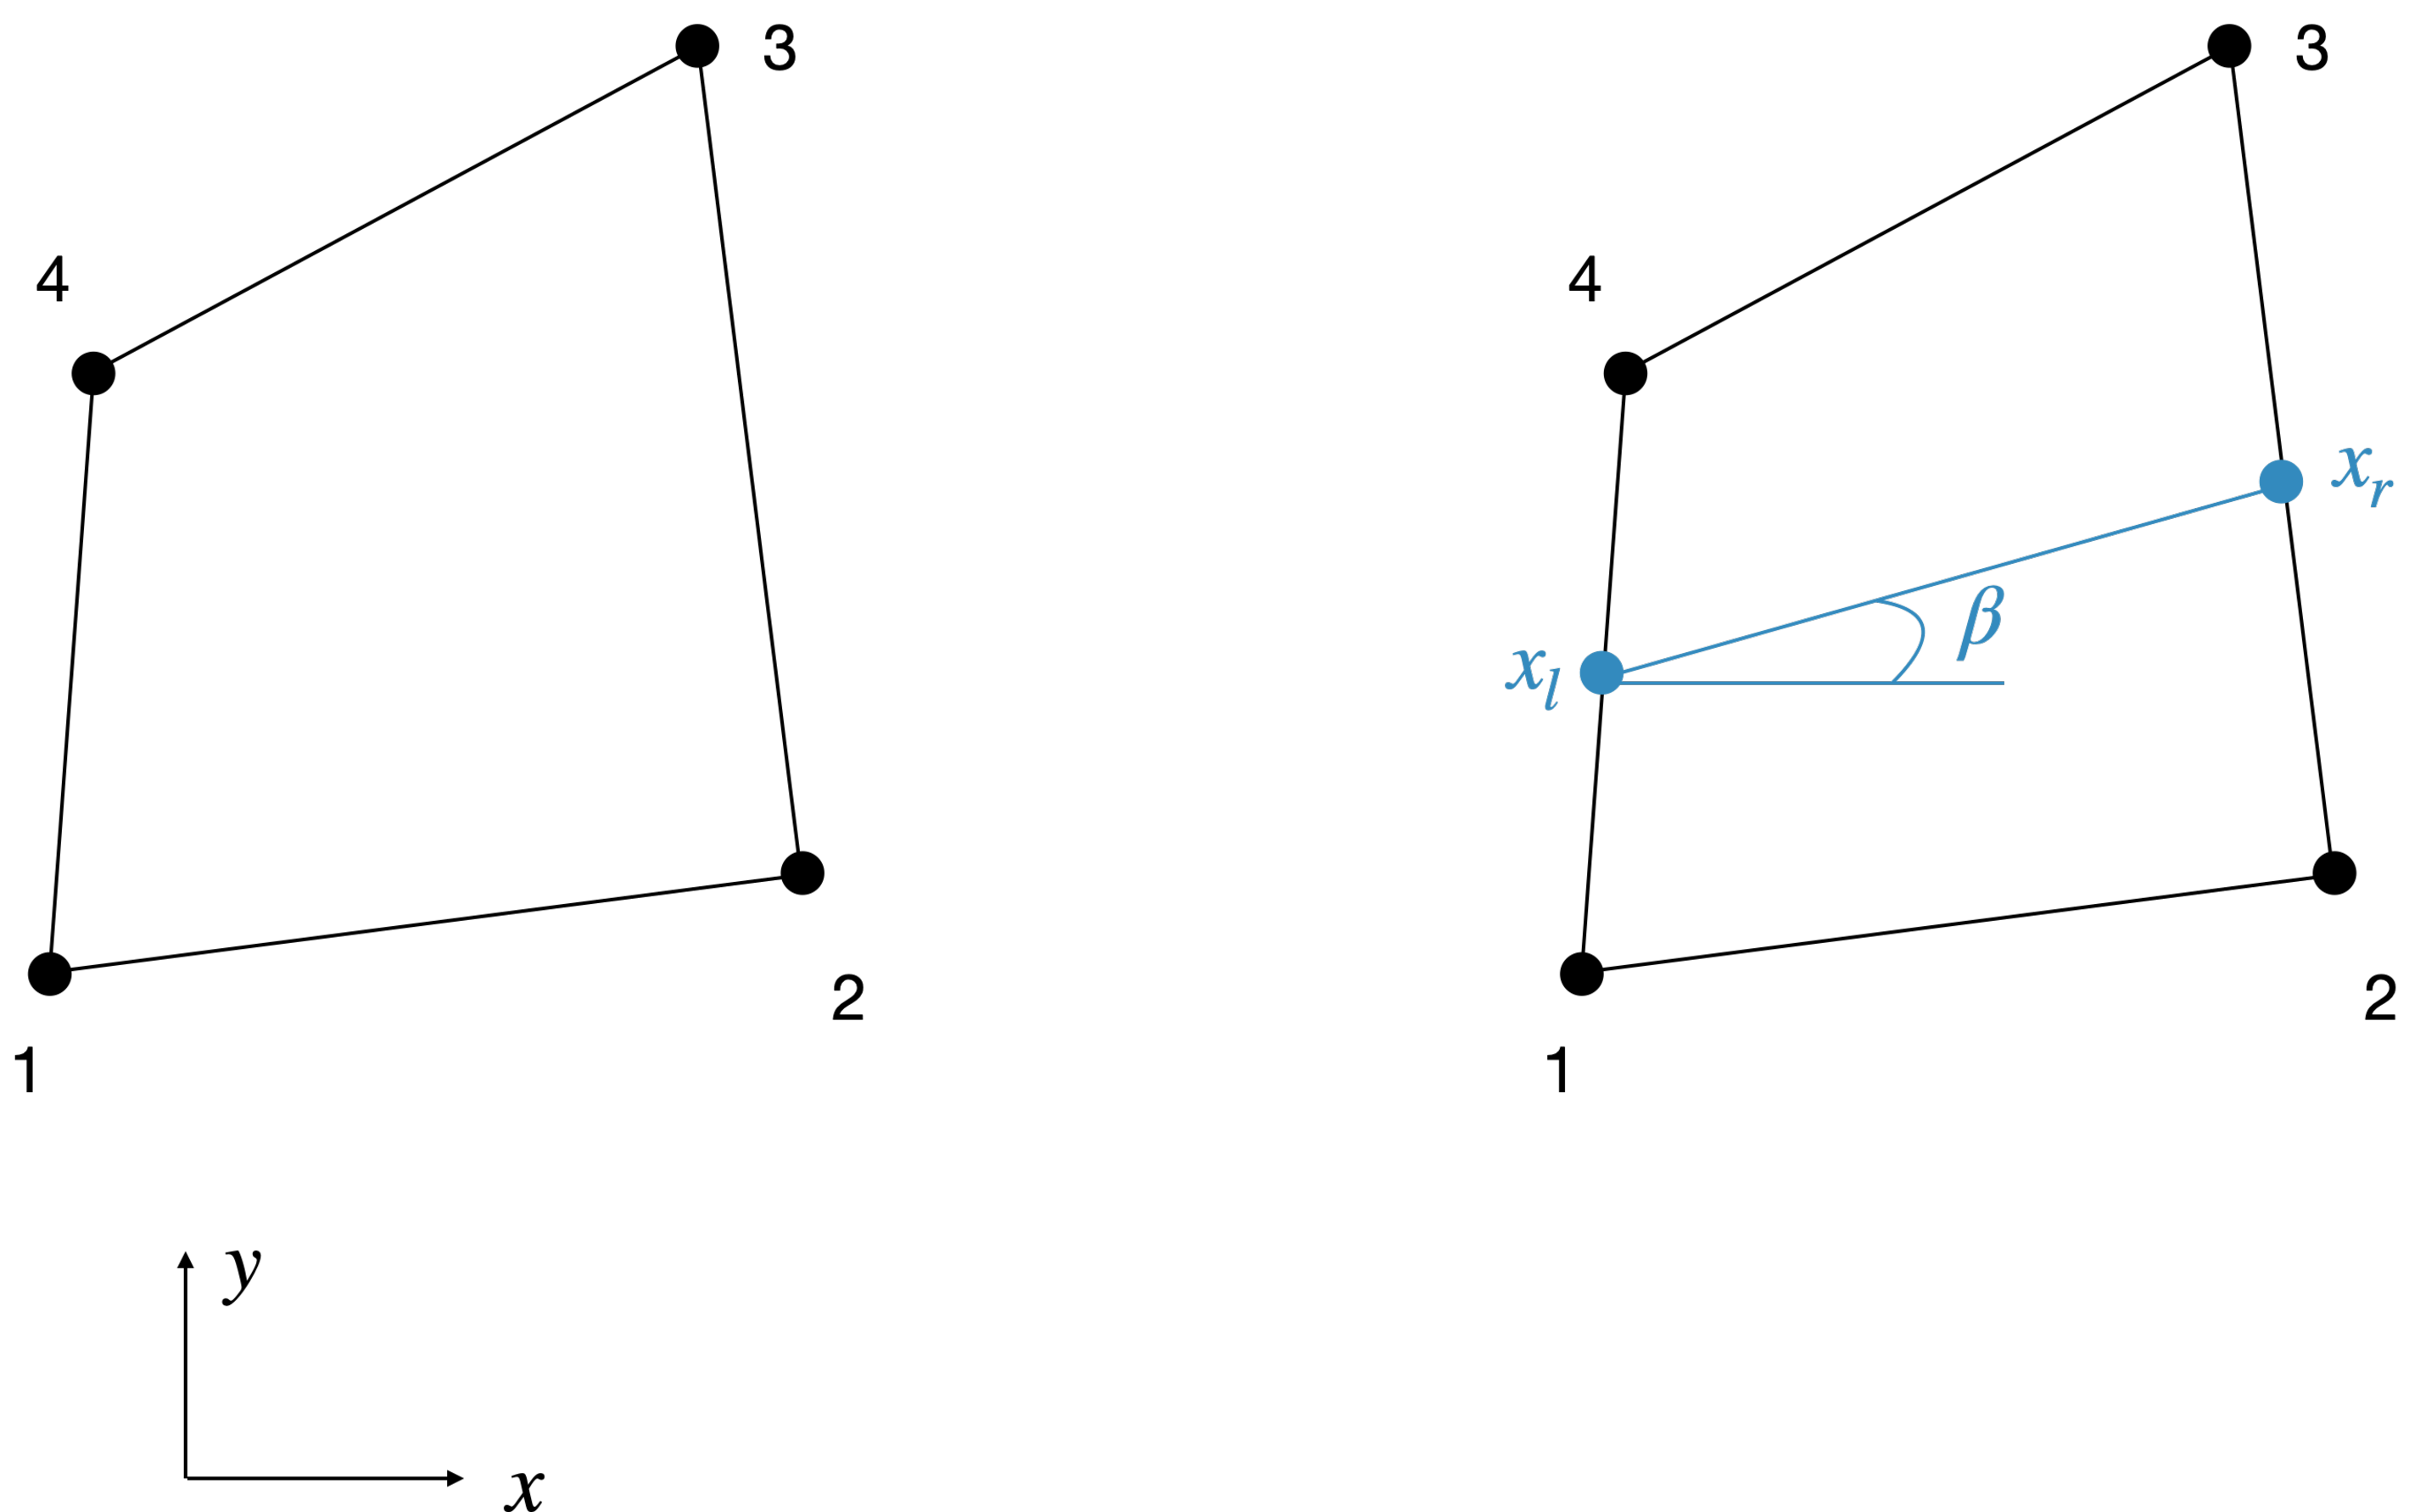
\includegraphics[width=4.0in]{element}
\caption{The order of nodes in an element.  Also shows $\beta$ as defined by the element geometry.}
\label{fig:element}
\end{figure}
Note that the angle of $\beta$ is not necessarily one value for an element when the sides are not parallel.  We average the top and bottom sides, and compute the angle from that line as shown on the right side of the figure.  The left point is given by:
\begin{equation}
\begin{aligned}
    x_l &= \frac{1}{2} (x_1 + x_4)\\
    y_l &= \frac{1}{2} (y_1 + y_4)
\end{aligned}
\end{equation}
whereas the right point is:
\begin{equation}
\begin{aligned}
    x_r &= \frac{1}{2} (x_2 + x_3)\\
    y_r &= \frac{1}{2} (y_2 + y_3)
\end{aligned}
\end{equation}

Rather than compute the angle $\beta$, we compute $\cos\beta$ and $\sin\beta$ directly to avoid any issues with obtaining the correct angle as the quadrant varies (atan2 could also work), and because it is $\cos\beta$ and $\sin\beta$ which we need anyway.
Observing the right hand side of \cref{fig:coordinate} we see that
\begin{equation}
\cos\beta = \frac{\Delta x}{\Delta s}
\end{equation}
and
\begin{equation}
\sin\beta = \frac{\Delta y}{\Delta s}
\end{equation}
where $\Delta x = x_r - x_l$, $\Delta y = y_r - y_l$, and $\Delta s = \sqrt{(\Delta x)^2 + (\Delta y)^2}$.


From this stage we use the approach developed by Giavotto et al.~\cite{Giavotto1983}.  This method was clearly expounded by Blasques in his user guide for the code BECAS \cite{Blasques2012}.  We do not repeat this derivation as it has been clearly derived in these previous documents.  However, the latter has a couple of typos, which are noted below.

First, the definition for the matrix $C$ changes in two different parts of the document (a transpose in the definition), which leads to some inconsistencies in the derivation.   We use the original definition from \cite{Giavotto1983}:
\begin{equation}
C = \int_A (BN)^T Q (SN) dA = \int_A (BN)^T Q (SN) |J| d\xi d\eta
\end{equation}

This transpose inconsistency, and also a sign error carried down improperly in one of the lines of the derivation changes this term:
\begin{equation}
\begin{bmatrix}
    (C - C^T) & L \\
    L^T & 0 \\
    0 & 0 \\
\end{bmatrix}
\end{equation}
to this:
\begin{equation}
\begin{bmatrix}
    (C^T - C) & L \\
    -L^T & 0 \\
    0 & 0 \\
\end{bmatrix}
\end{equation}

After computing the compliance and stiffness matrices, we reorder them to GXBeam format.



\bibliographystyle{aiaa}
\bibliography{sectionprop}

\end{document}

